\chapter{Estado del arte}
\label{cap:arte}

\section{Aplicaciones similares y comparativas}
\label{sec:aplicaciones}

\subsection{Tricount}
\label{subsec:tricount}

Tricount es una aplicación diseñada para facilitar la gestión y el reparto de gastos entre varias personas. Es útil en sistuaciones,
donde un grupo de personas realiza gastos comunes, como en viajes o cenas. Es una aplicación bastante sencilla de usar, lo que la 
hace aún más popular entre los grupos de personas. Está disponible para Android e iOS y tiene también soporte web. 

\subsubsection{Funciones Principales}
\label{subsubsec:funciones}
\begin{enumerate}
    \item \textbf{Creación de un Tricount}
    \begin{enumerate}
        \item Configuración Inicial. Al iniciar un nuevo "Tricount" (grupo) se le da un nombre, se elige un tipo de divisa y se añade a los participantes.
        \item Acceso Compartido. Puede ser compartido entre todos los participantes a través de un enlace, lo que permite que cada uno pueda añadir sus gastos.
    \end{enumerate}
    \item \textbf{Añadir Gastos}
    \begin{enumerate}
        \item Registro de Gastos. Cualquier participante puede añadir un gasto en el tricount, especificando la cantidad, la categoría,
        quien pagó y para quien es ese gasto.
        \item División Personalizada. Tricount permite dividir los gastos de forma equitatica o personalizada, es decir, si el gasto es para todos o solo para algunos. 
        \item Comentarios. Se pueden añadir comentarios a cada pago.
    \end{enumerate}
    \item \textbf{Cálculo Automático}
    \begin{enumerate}
        \item Resumen de Balances. Se calcula automáticamente cúanto debe cada persona y a quien. 
        \item Balances Individuales. Cada participante puede ver su valance individual y cuánto ha gastado, cuánto le deben y cuánto le debe a otros.
    \end{enumerate}
    \item \textbf{Saldar Deudas}
    \begin{enumerate}
        \item Recomendaciones de Pagos. Tricount recomienda la mejor manera de saldar las deudas dentro del grupo, optimizando el número de 
        transsaciones necesarias.
        \item Pagos Parciales o Totales. Los participantes puedden registrar pagos parciales o totales dentro de la aplicación para mantener un
        seguimiento claro de lo que ha sido pagado y lo que queda pendiente.
    \end{enumerate}
\end{enumerate}

\subsubsection{Modo de Uso}
Una vez nos hayamos descargado la aplicación ya sea desde Google Play o App Store, lo primero 
que nos muestra es una pantalla de inicio como nos muestra la \textit{Figura \ref{principal}}.

\begin{figure}[ht]
    \centering
    \begin{minipage}{0.45\textwidth}
        \centering
        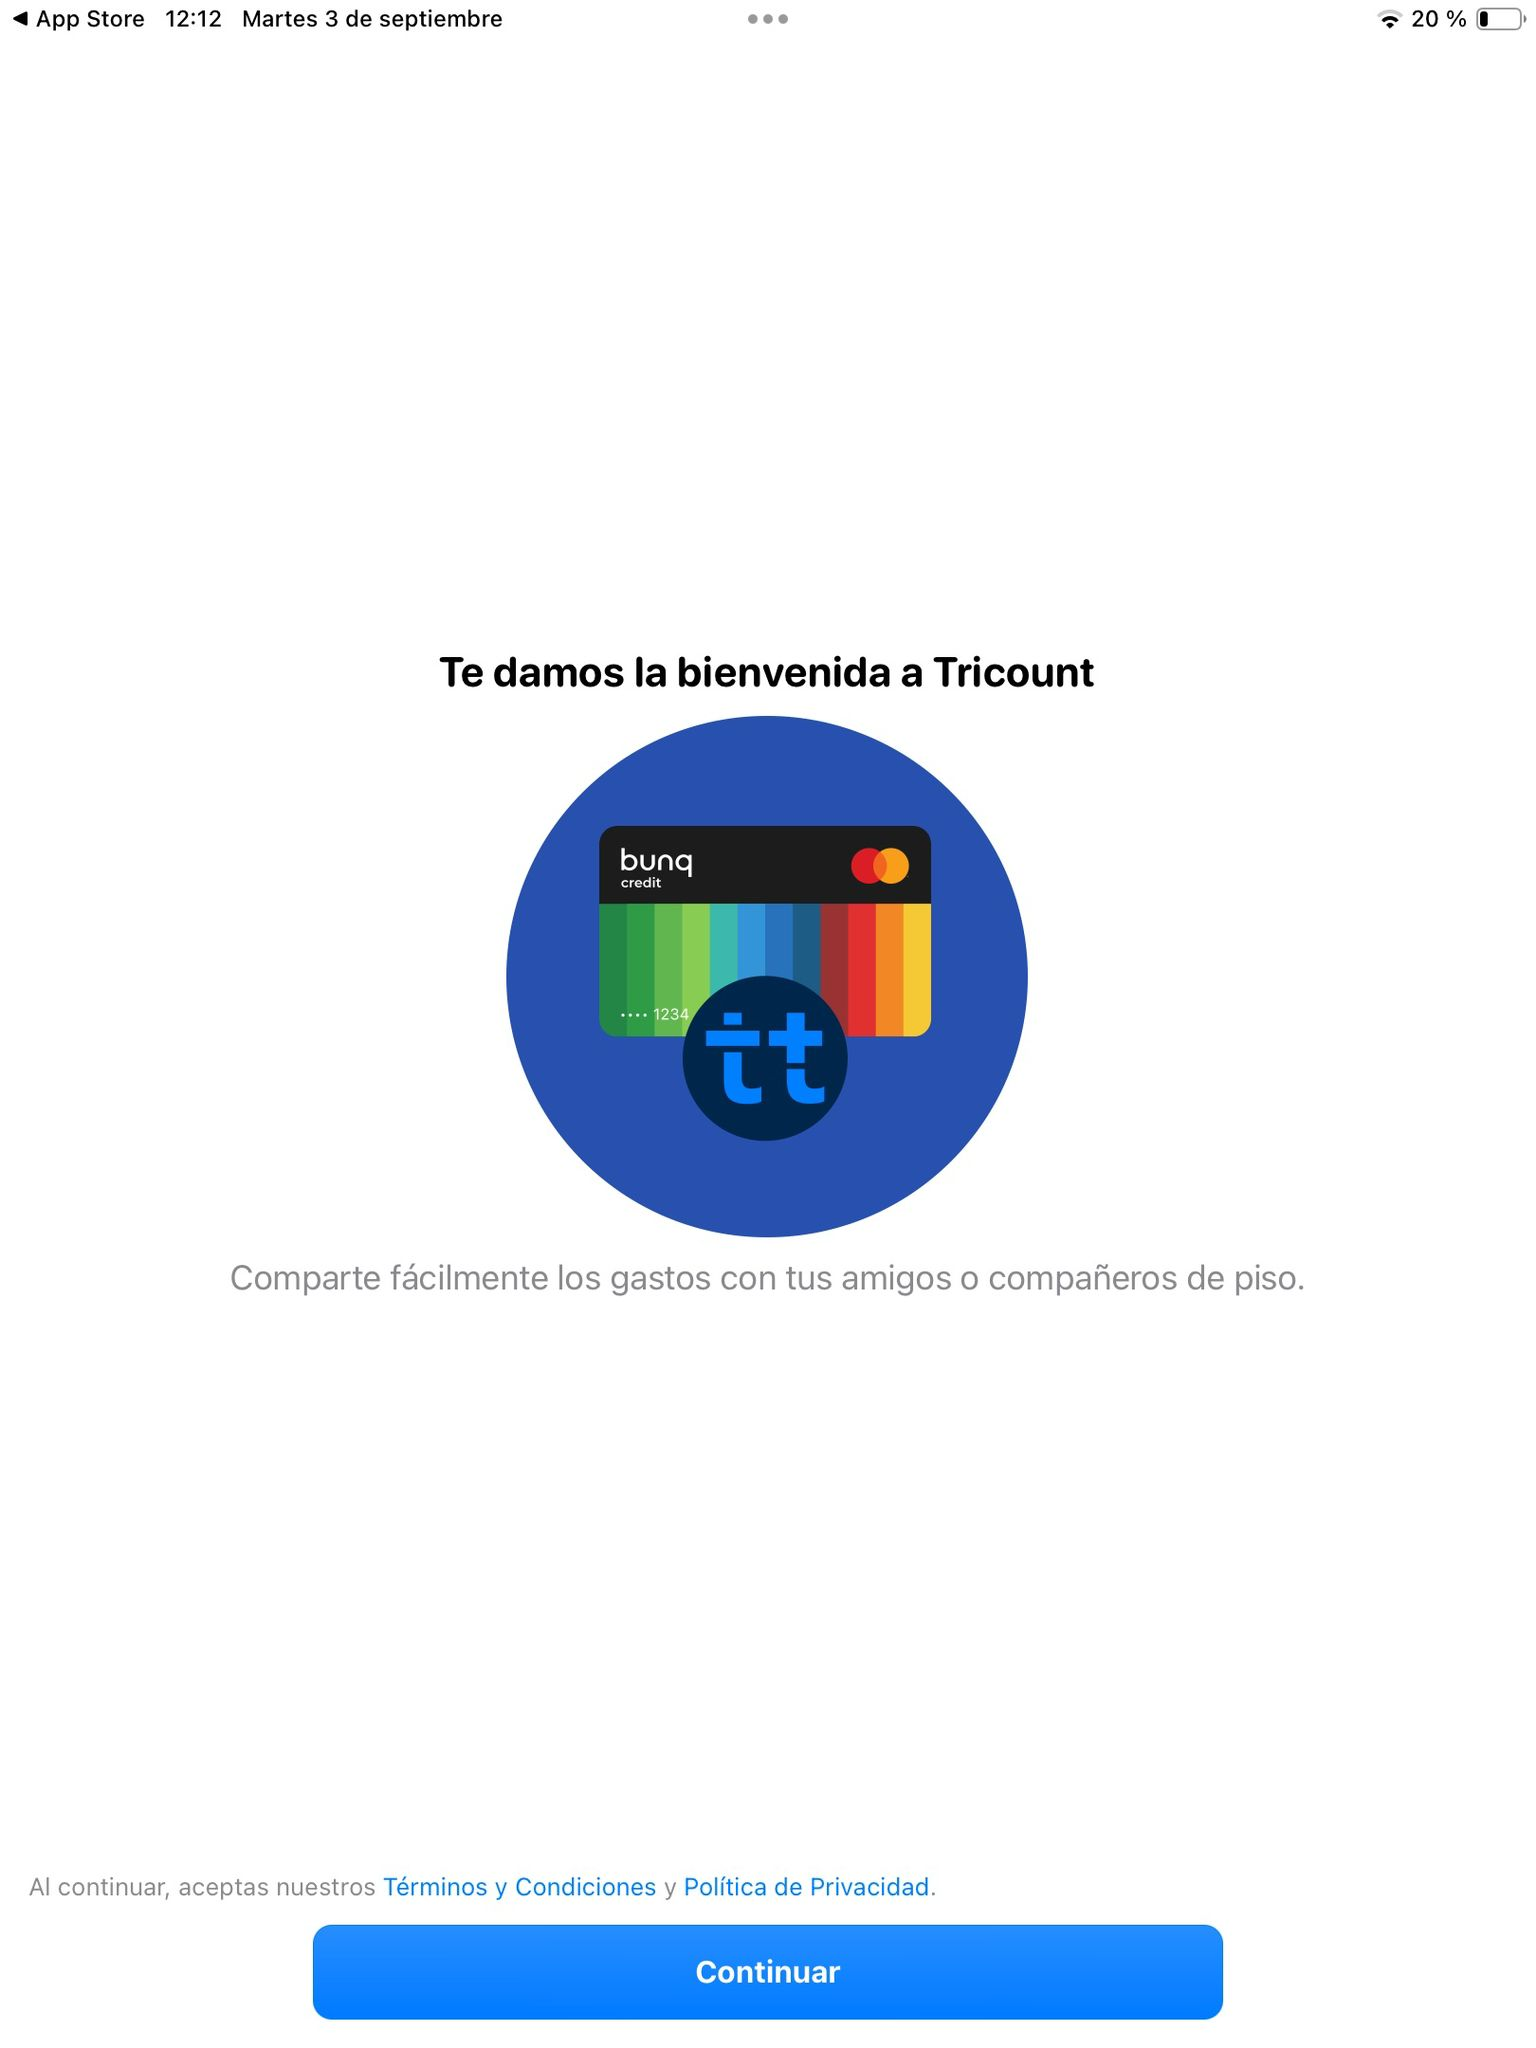
\includegraphics[width=\textwidth]{../capitulos/img/principal.jpg}
        \caption{Pantalla Inicio.}
        \label{principal}
    \end{minipage}
    \hfill
    \begin{minipage}{0.45\textwidth}
        \centering
        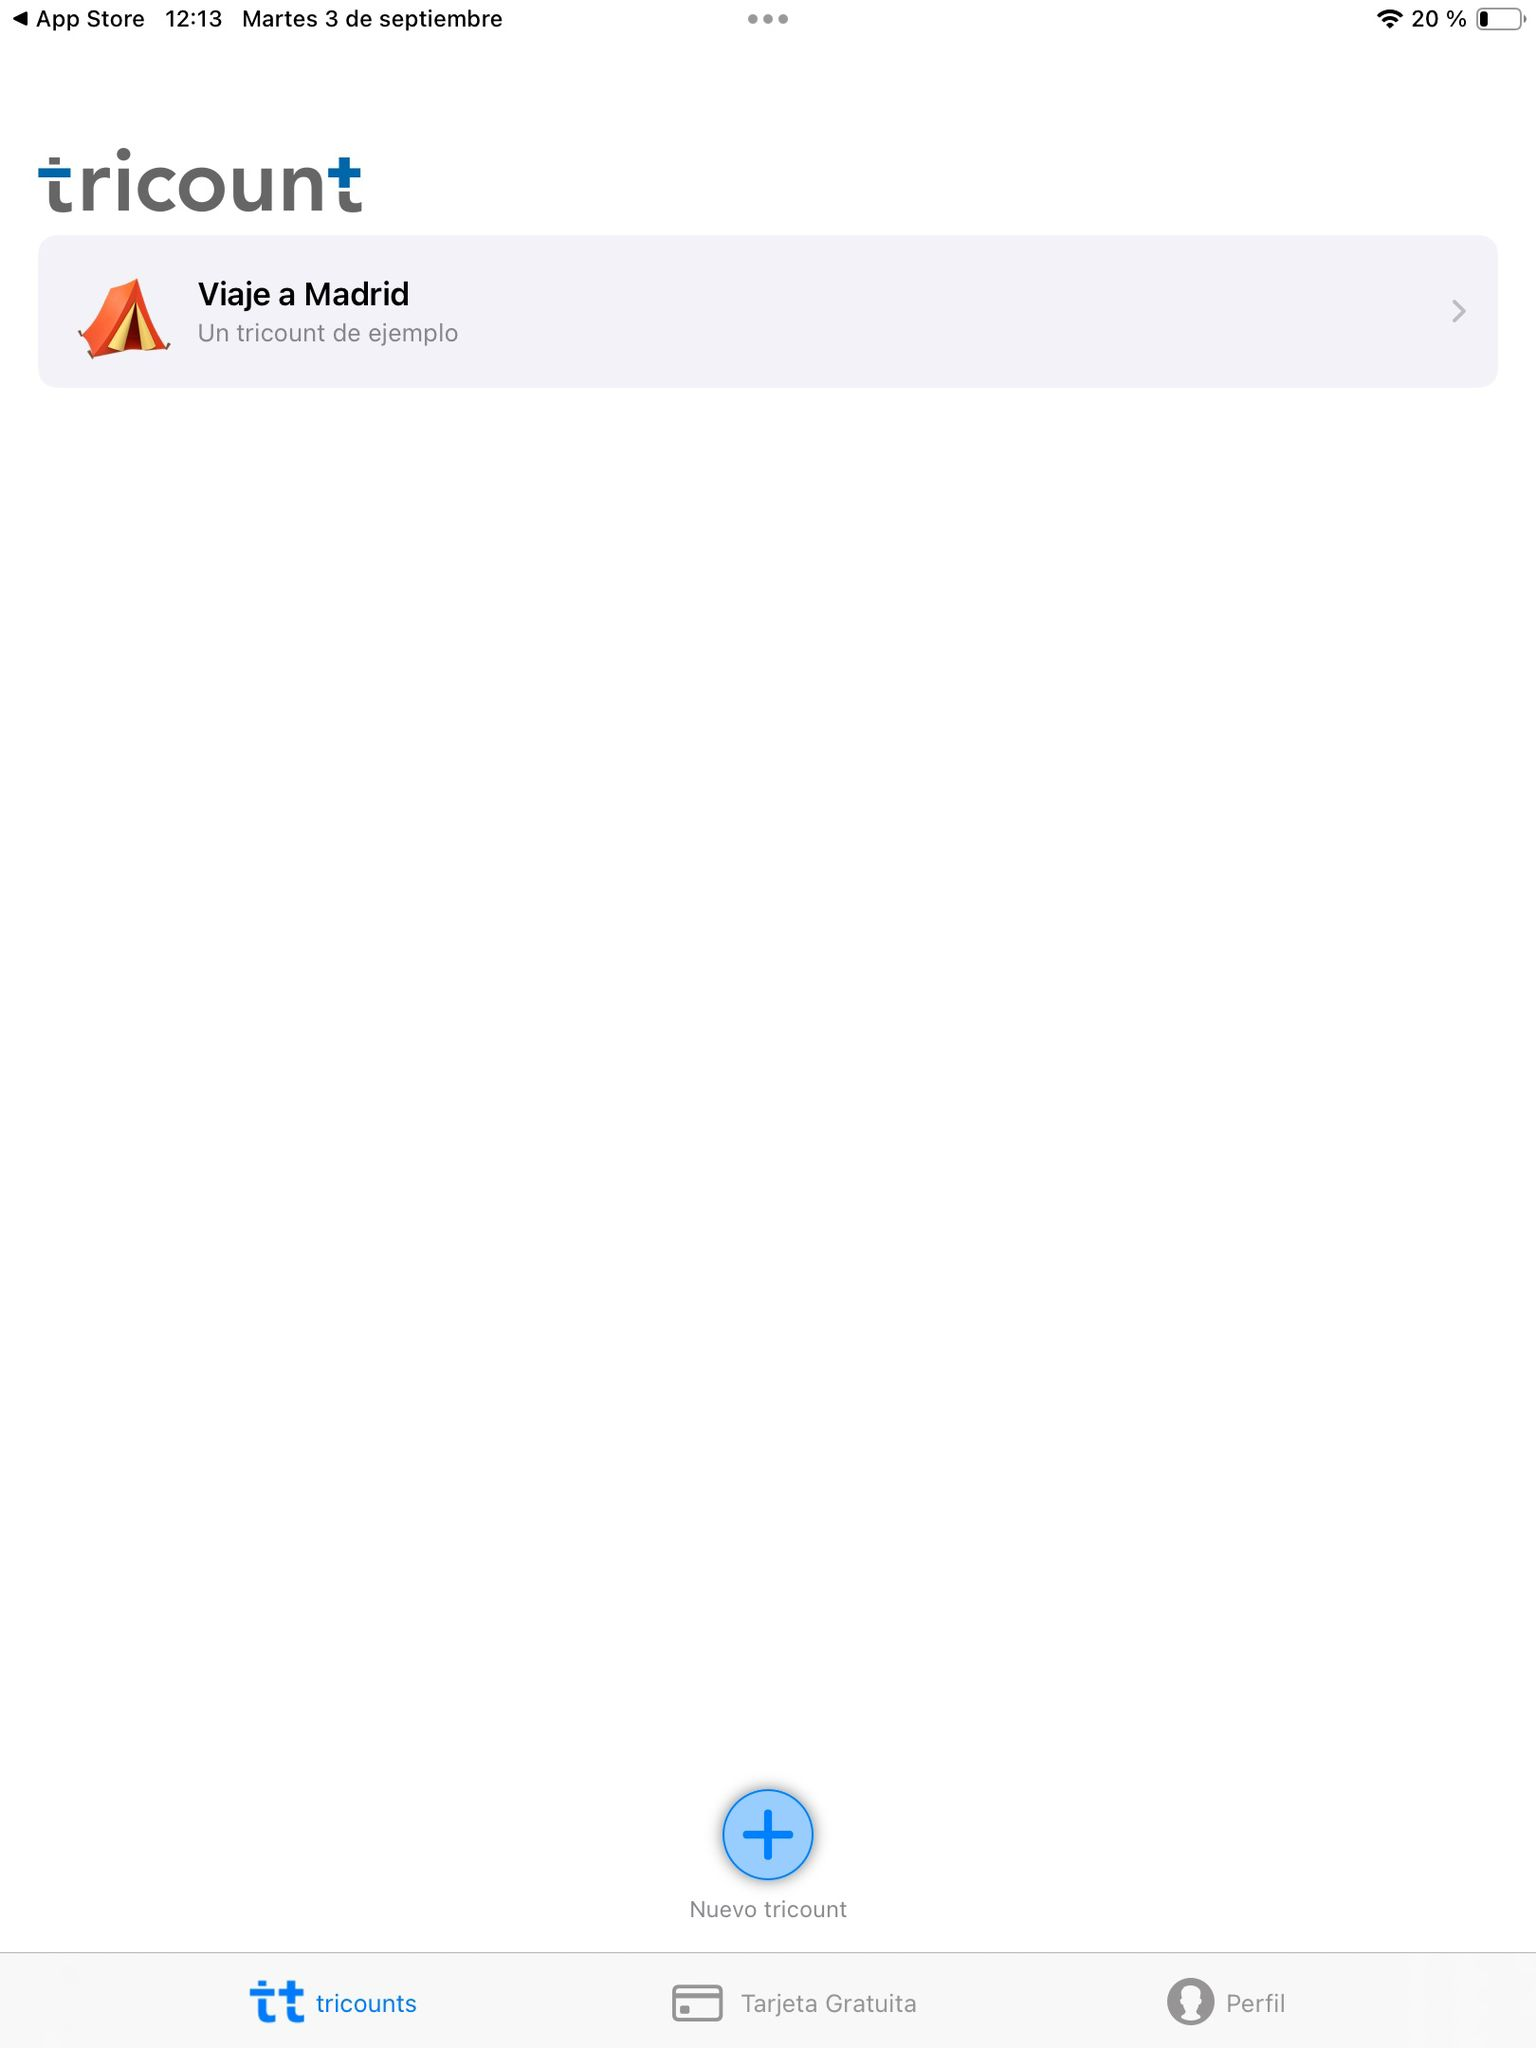
\includegraphics[width=\textwidth]{../capitulos/img/inicio.jpg}
        \caption{Lista de grupos.}
        \label{grupos}
    \end{minipage}
\end{figure}



Pulsado el botón de \textit{Continuar} nos muestra una pantalla donde 
nos sale una lista de los grupos que hemos creado o en los que estamos participando.
En este caso como es la primera vez que entramos solo nos muestra un grupo de ejemplo
(\textit{Figura \ref{grupos}}).


Para añadir un nuevo grupo, pulsamos el botón de \textit{Nuevo Tricount} 
y nos muestra una pantalla emergente donde nos da dos opciones, la primera 
es iniciar un Tricount (grupo) desde 0 y la otra es unirnos a un grupo ya existente (\textit{Figura \ref{nuevo}}).

\begin{figure}[ht]
    \centering
    \begin{minipage}{0.45\textwidth}
        \centering
        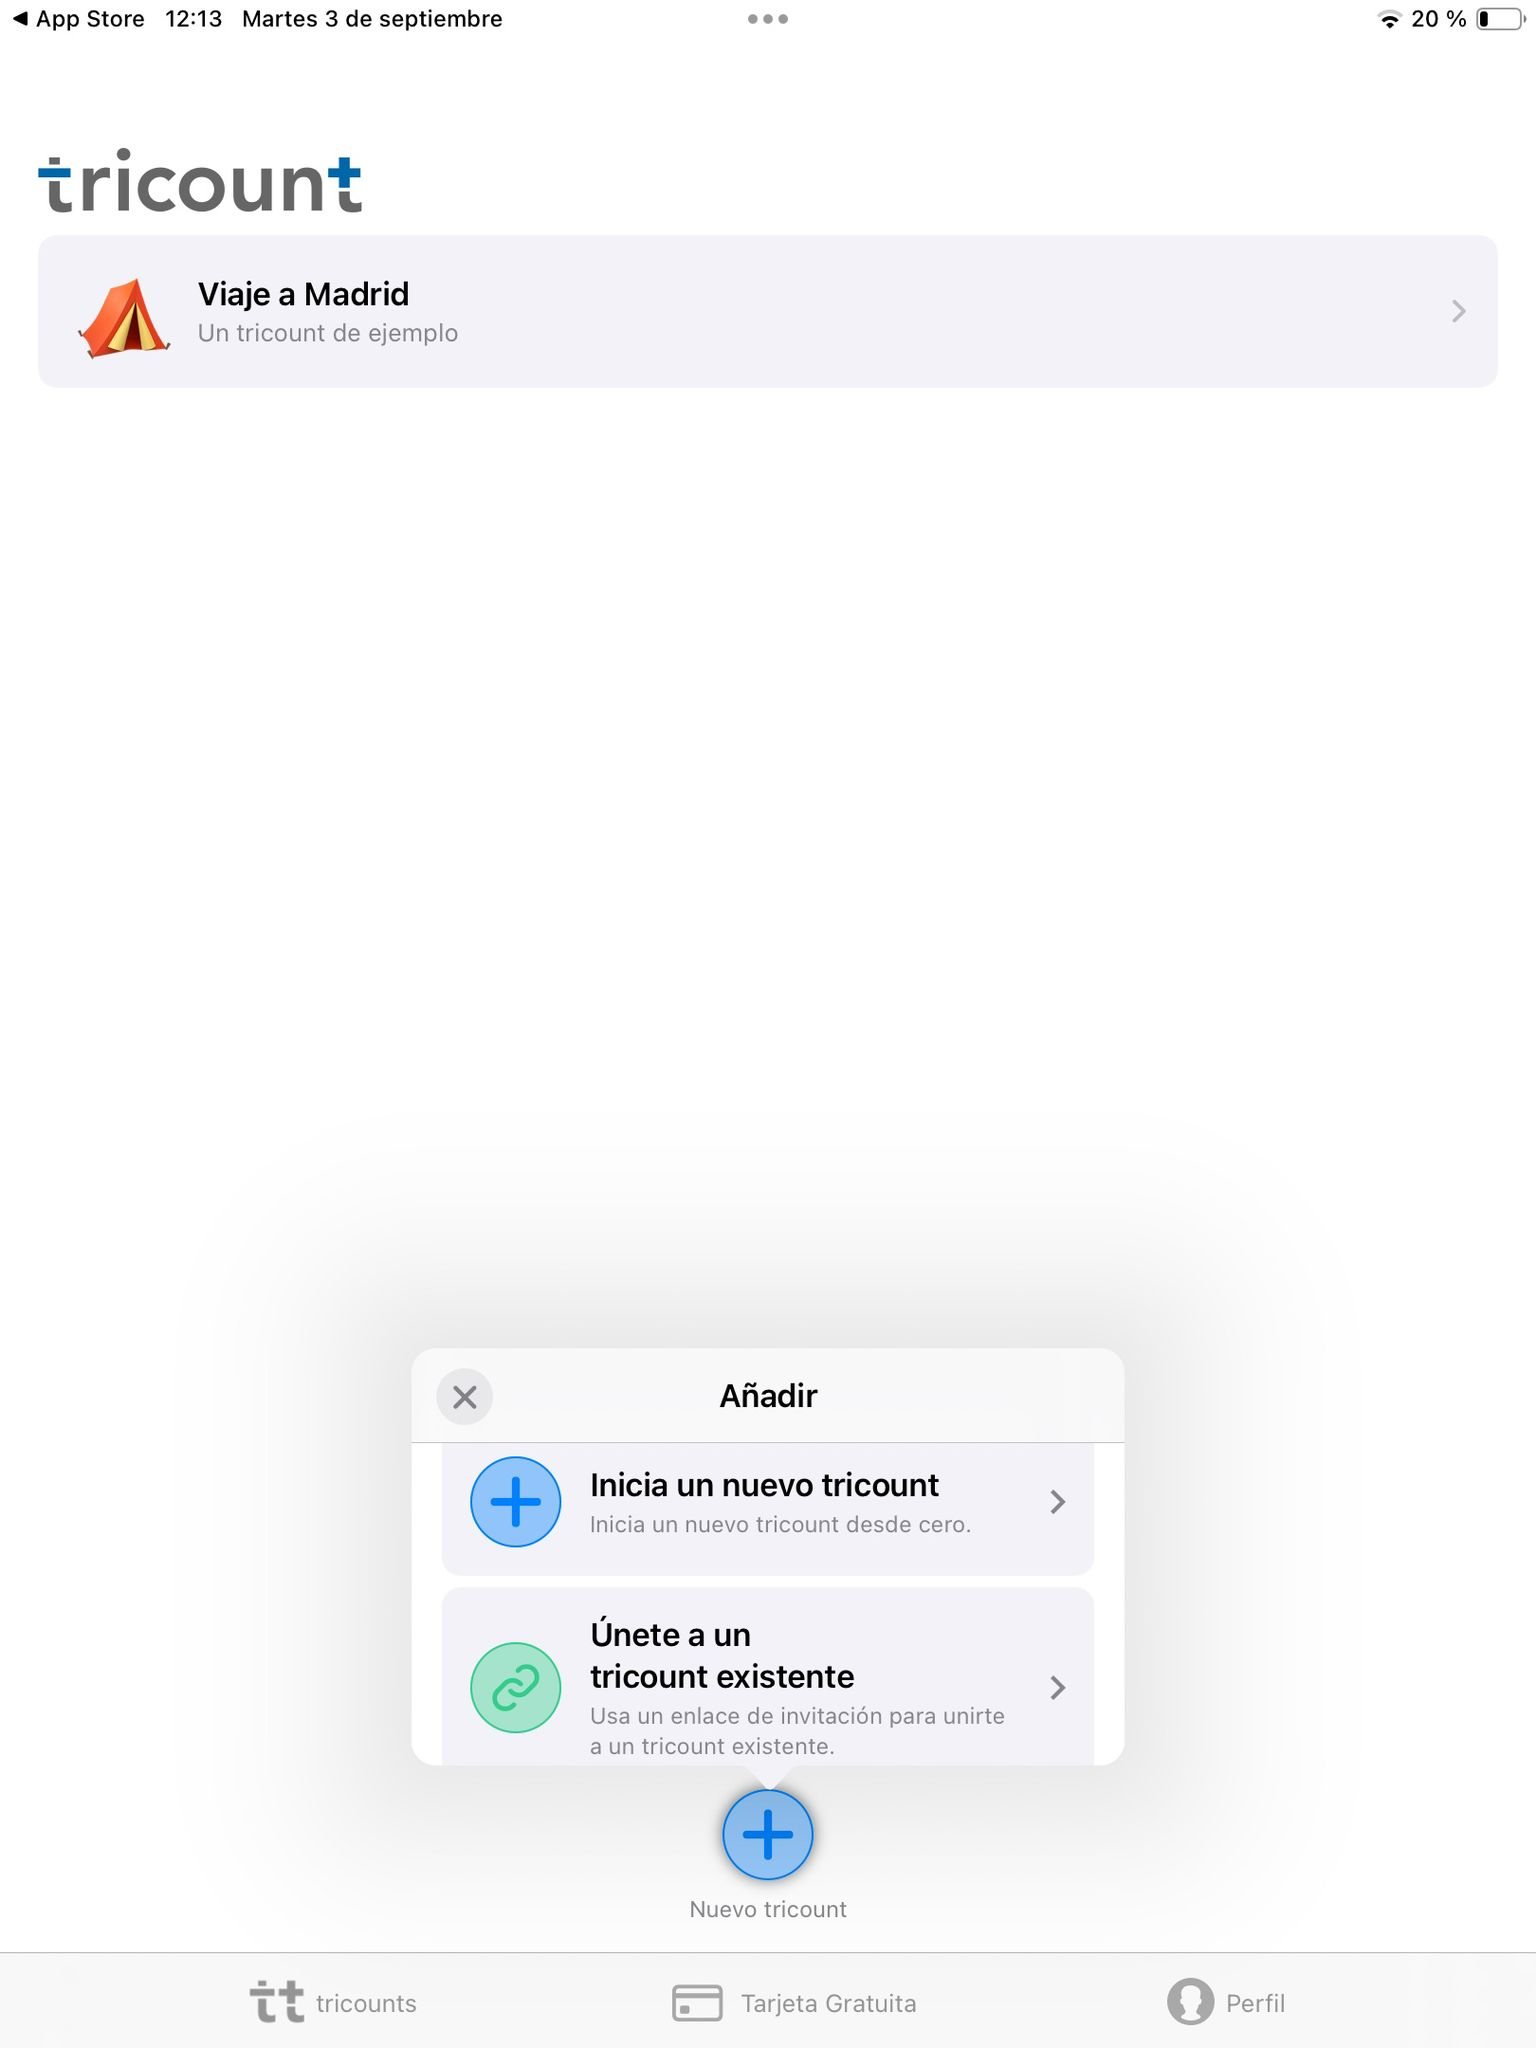
\includegraphics[width=\textwidth]{../capitulos/img/añadir.jpg}
        \caption{Añadir un nuevo grupo.}
        \label{nuevo}
    \end{minipage}
    \hfill
    \begin{minipage}{0.45\textwidth}
        \centering
        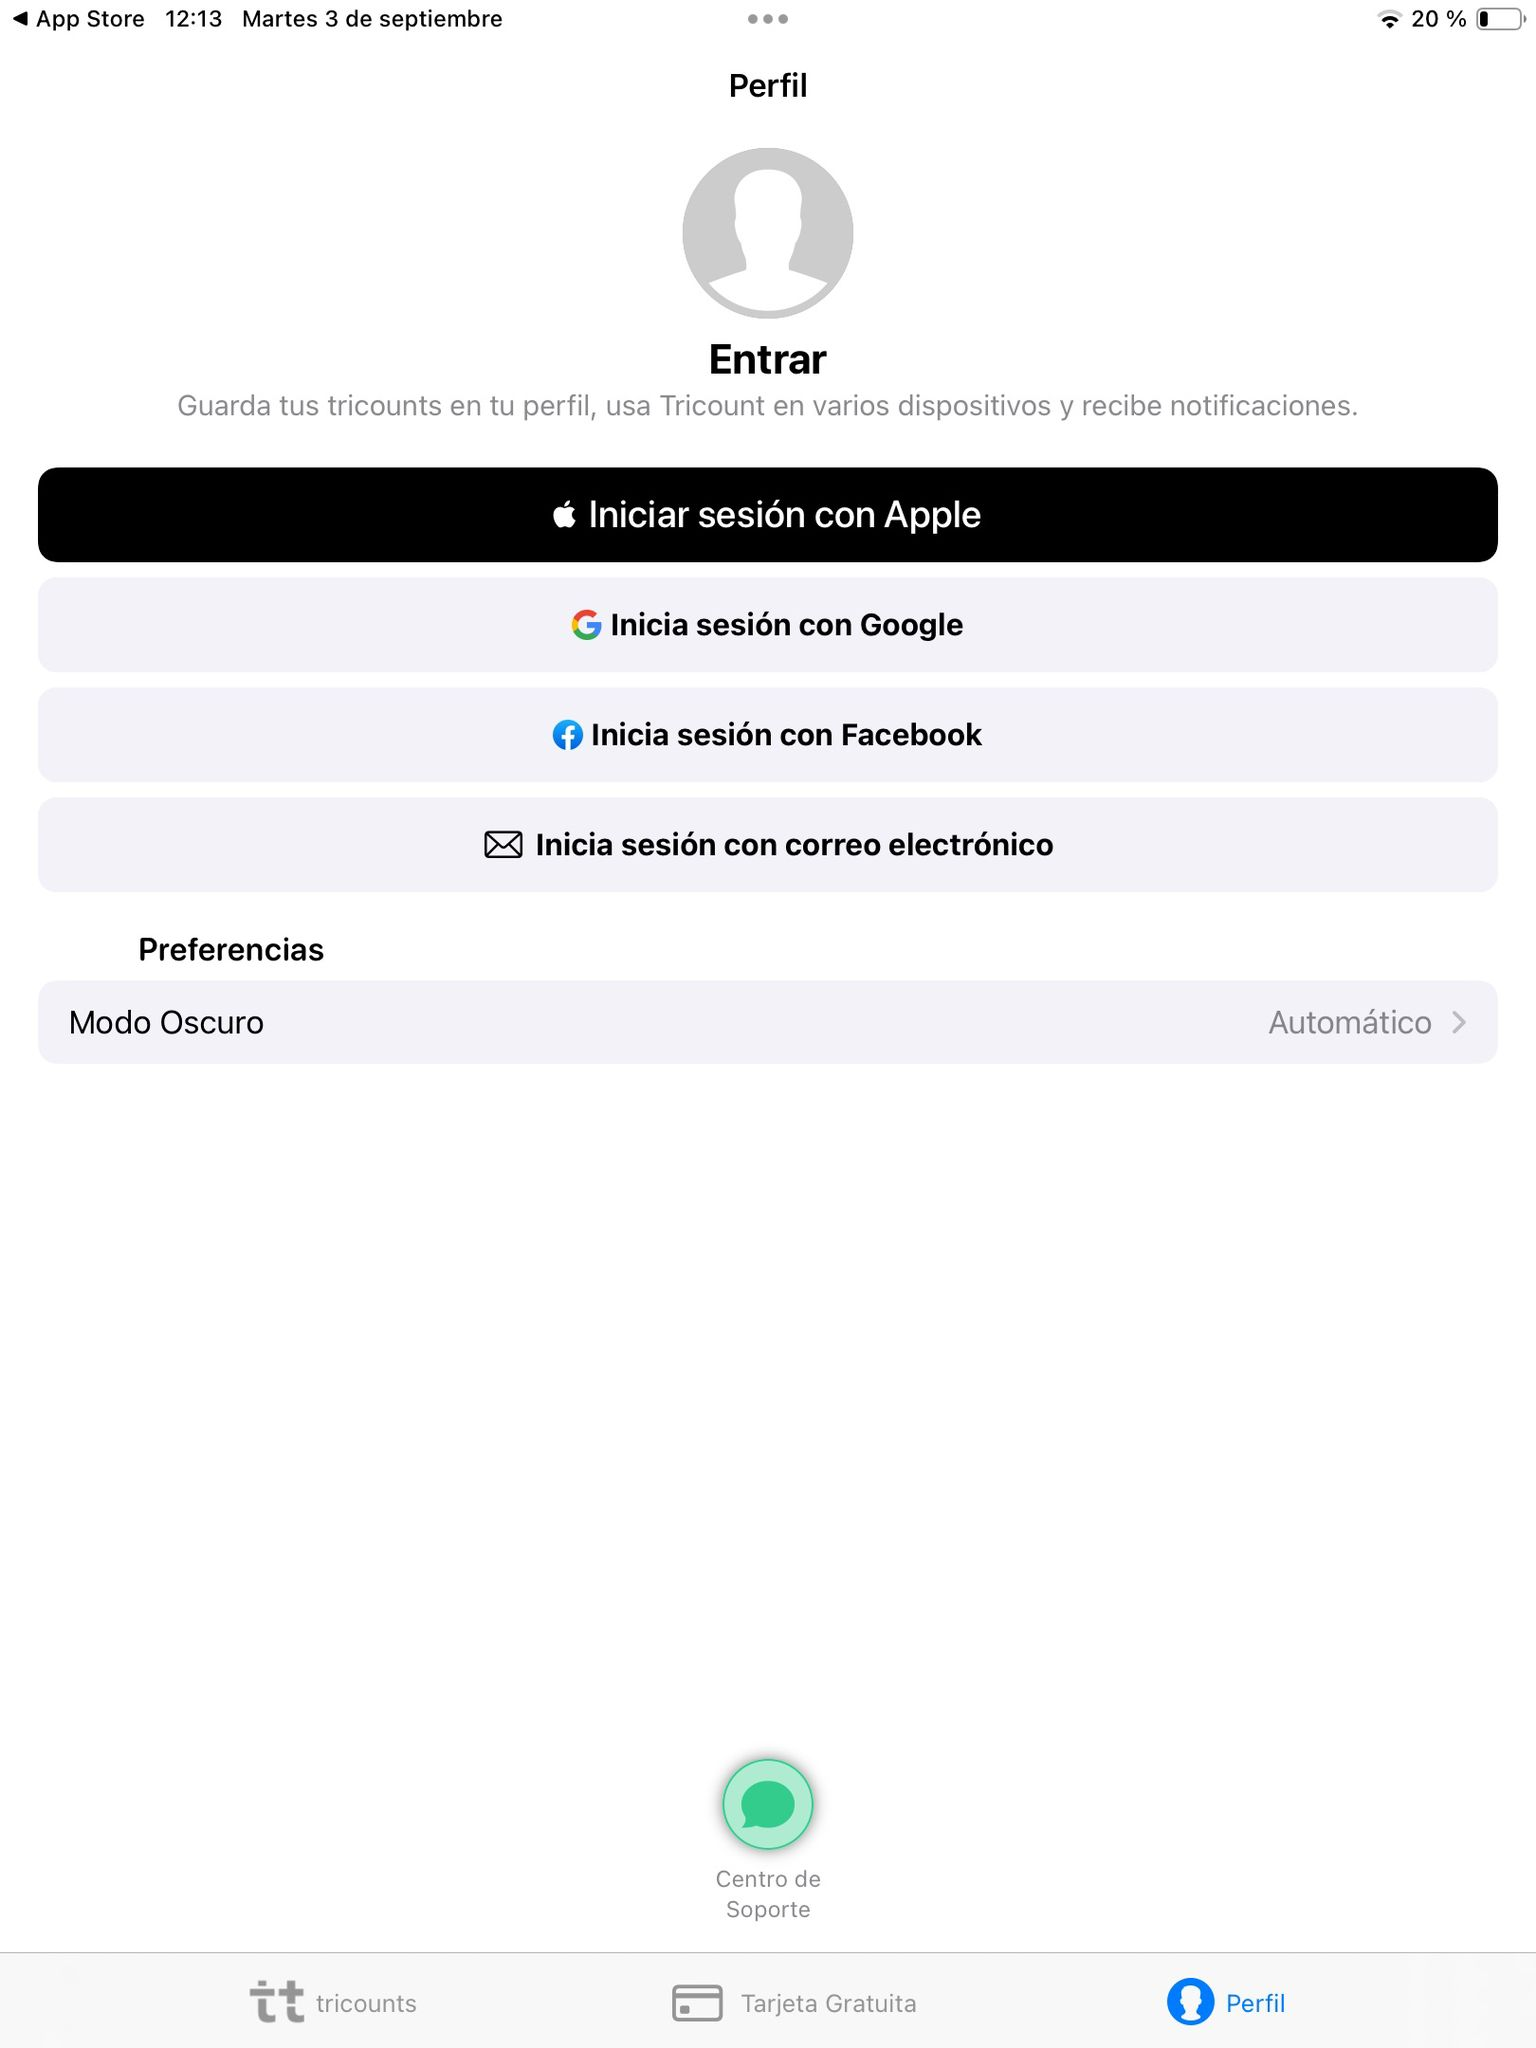
\includegraphics[width=\textwidth]{../capitulos/img/incio_sesion.jpg}
        \caption{Pantalla del perfil.}
        \label{perfil}
    \end{minipage}
\end{figure}


Otra de las pestañas que nos muestra es la del perfil, donde nos permite iniciar sesión y en caso de que ya estuvisemos registrado, 
se nos importan todos los grupos que estuvieran asociados a nuestra cuenta (\textit{Figura \ref{perfil}}). 
Ahora vamos a hablar de lo realmente importante de la aplicación y es de cómo crear un grupo y añadir gastos. Para ello después de 
pulsar el botón de \textit{Nuevo Tricount} nos da la opción de crear  un grupo desde 0, le damos un nombre, añadimos los miembros que van a
participar en el grupo y elegimos la divisa.(\textit{Figura \ref{crear_grupo}}). Una vez creado nos permite enviar un enlace a la gente que va a participar en el grupo
(\textit{Figura \ref{enlace}}).

\begin{figure}[ht]
    \centering
    \begin{minipage}{0.45\textwidth}
        \centering
        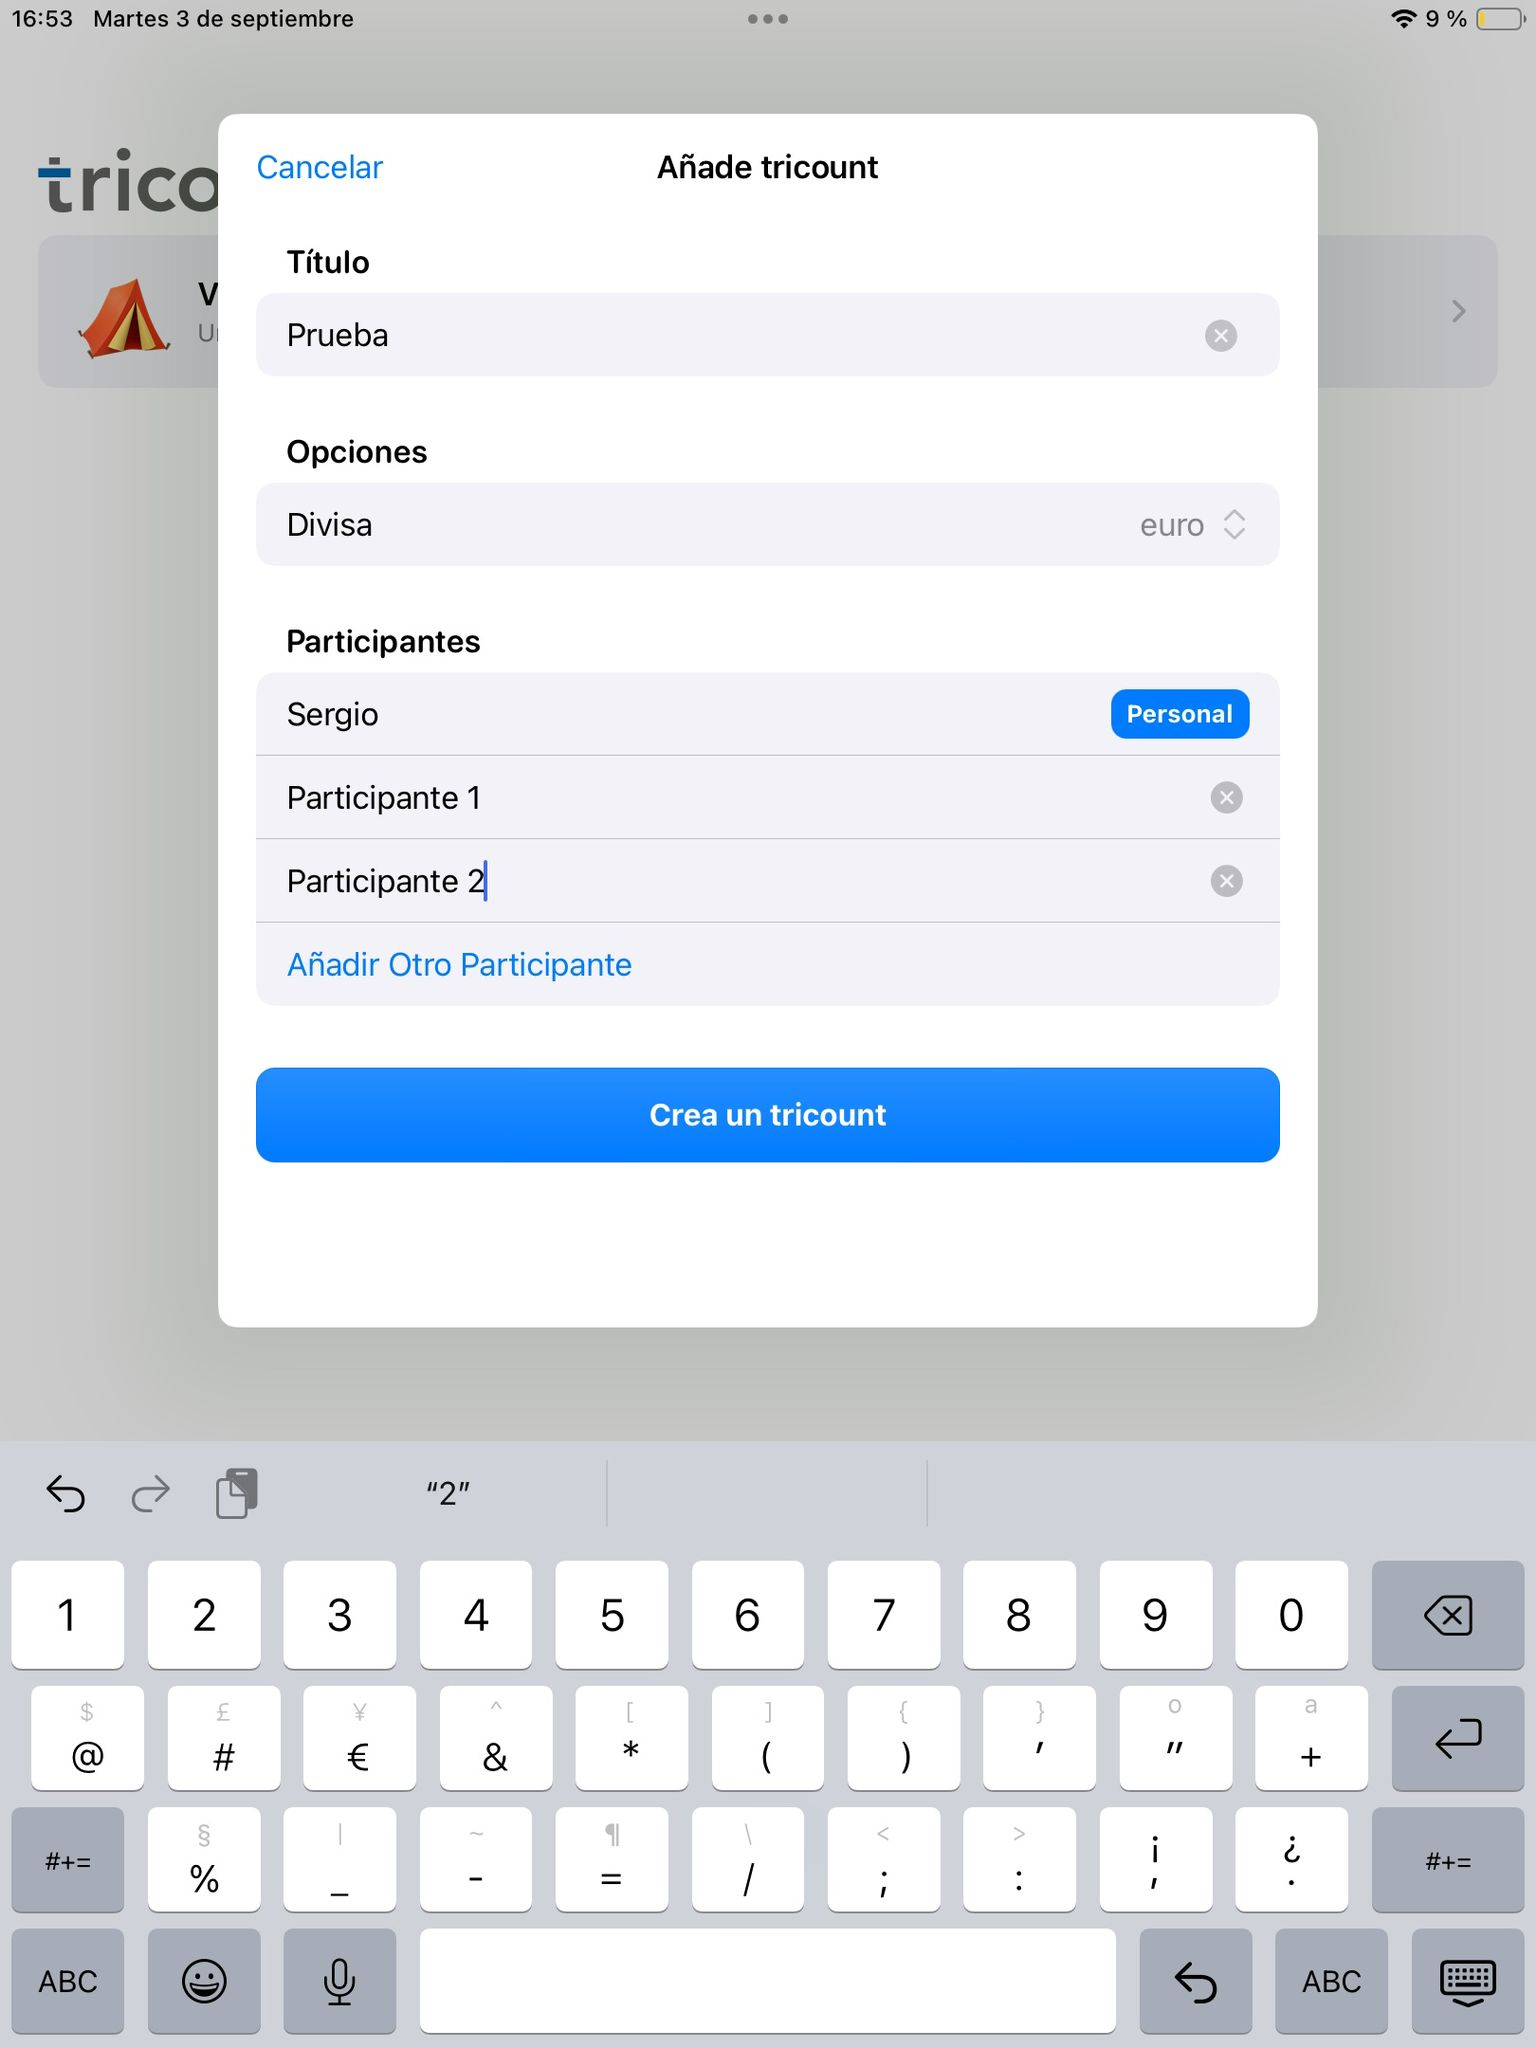
\includegraphics[width=\textwidth]{../capitulos/img/crear.jpg}
        \caption{Detalles de un nuevo grupo.}
        \label{crear_grupo}
    \end{minipage}
    \hfill
    \begin{minipage}{0.45\textwidth}
        \centering
        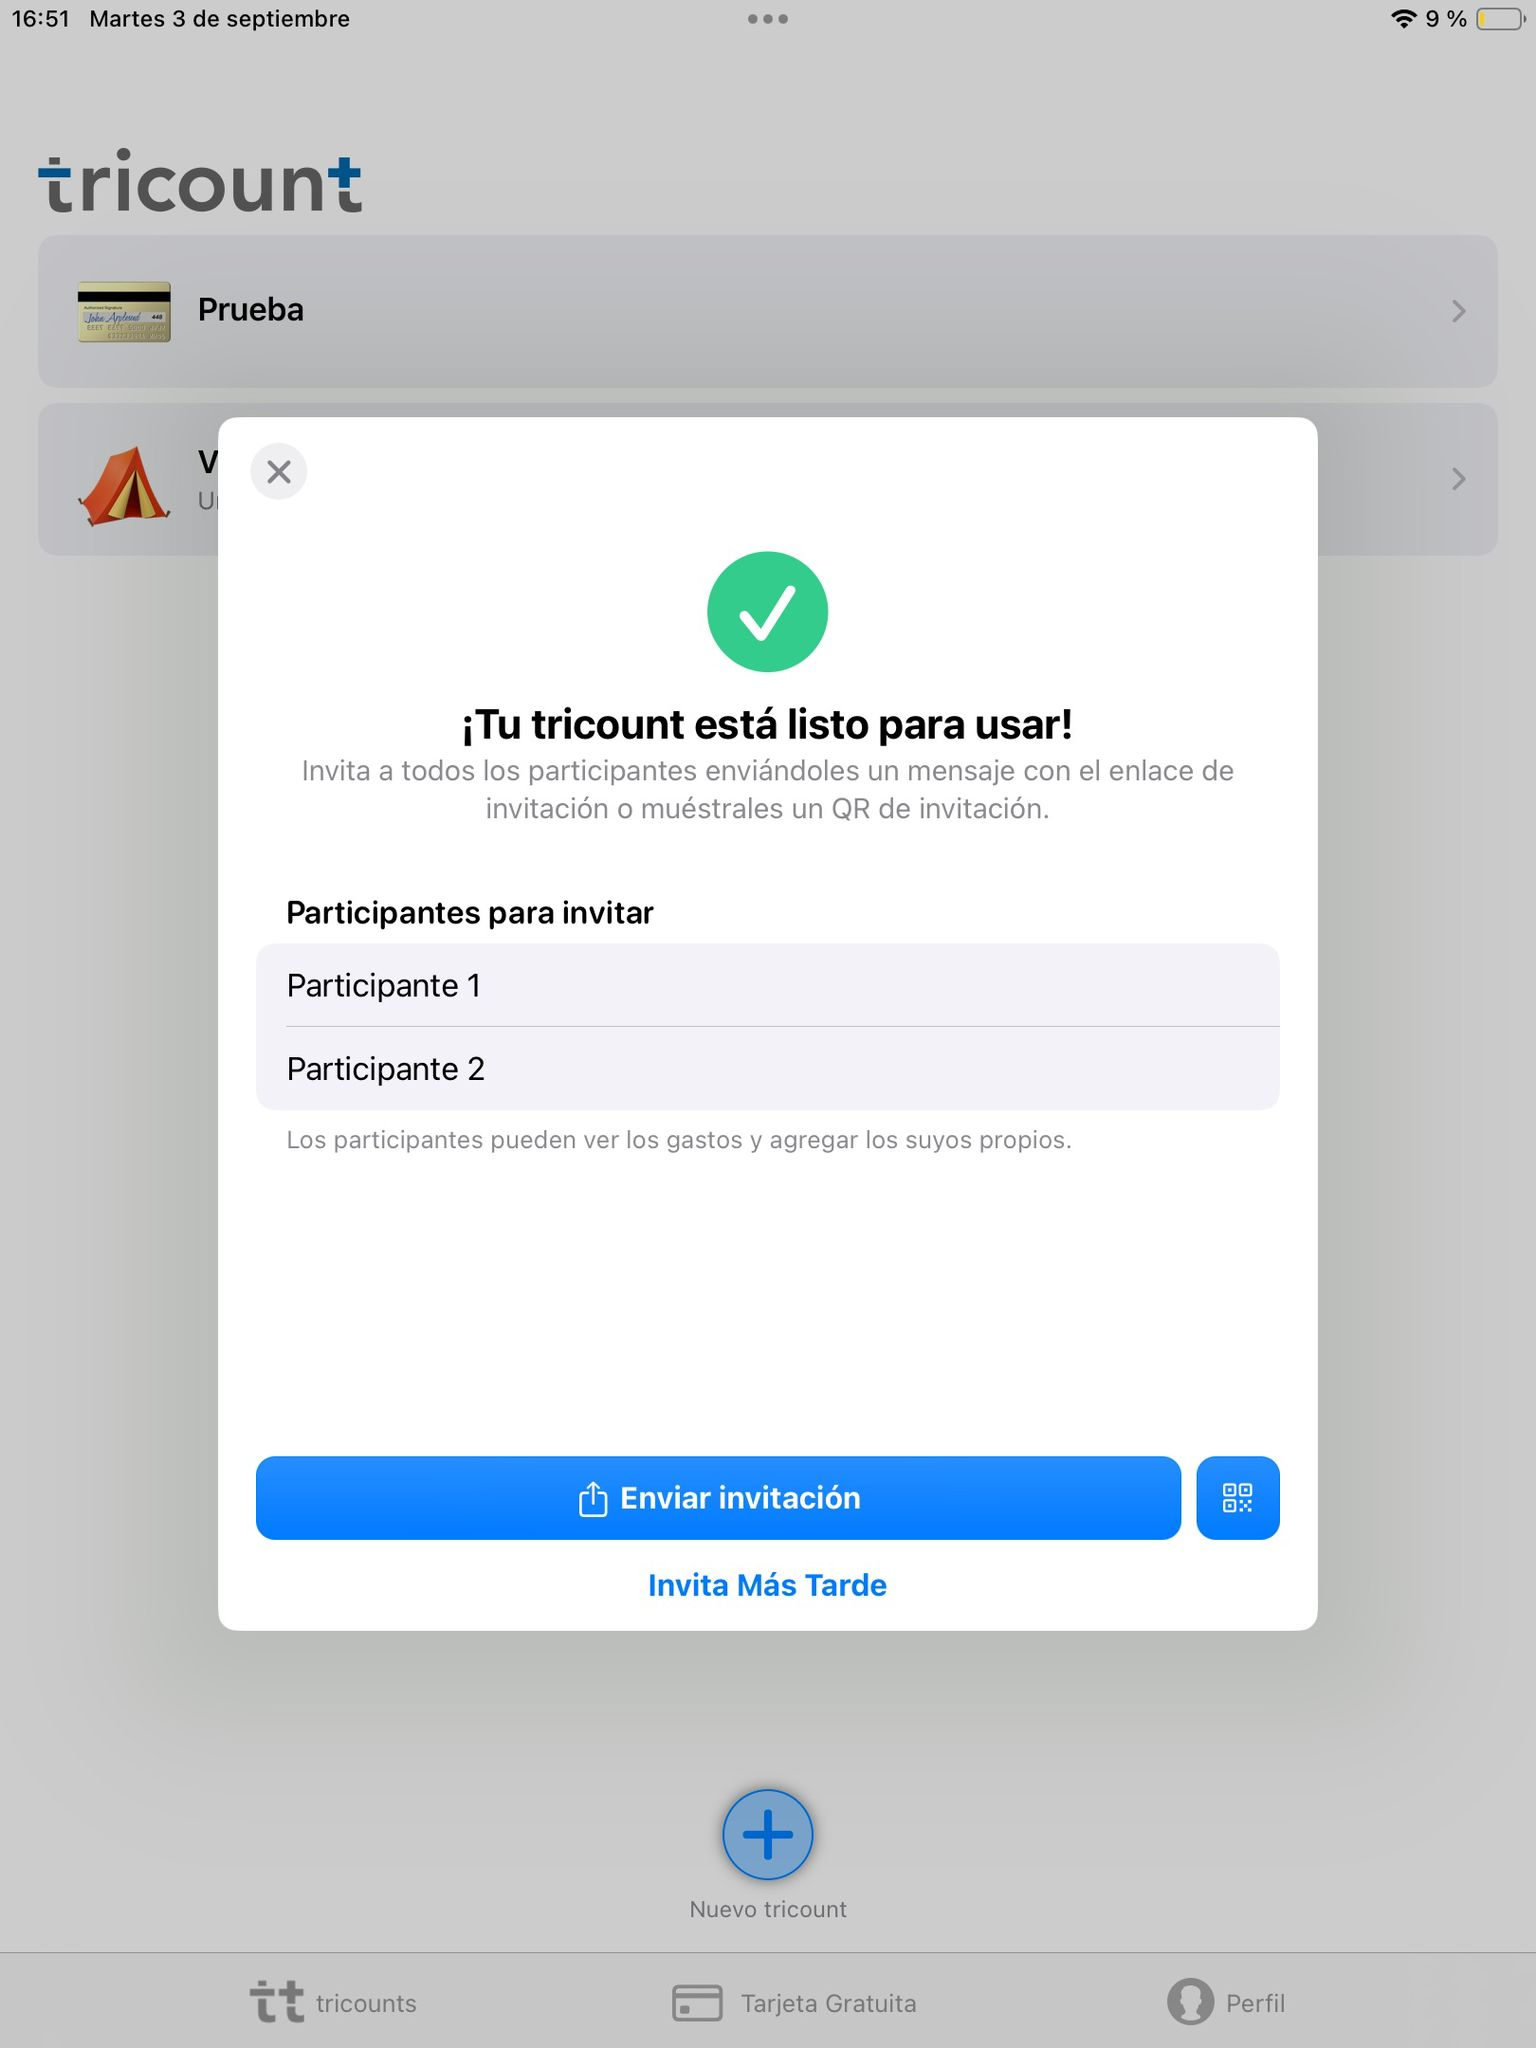
\includegraphics[width=\textwidth]{../capitulos/img/creado.jpg}
        \caption{Enviar invitación a los miembros del grupo.}
        \label{enlace}
    \end{minipage}
\end{figure}


Lo siguiente que vamos a hacer es añadir un gasto, para ello pulsamos el botón de \textit{Añadir un gasto}
y nos muestra una pantalla donde podemos añadir el nombre del gasto, la cantidad, la fecha, quien ha realizado 
el pago y a quien le corresponde pagar (\textit{Figura \ref{participantes}}). Por último, nos muestra un resumen de los gastos que se han realizado y las deudas que tiene cada miembro del grupo 
(\textit{Figura \ref{resumen}}).

\begin{figure}[ht]
    \centering
    \begin{minipage}{0.45\textwidth}
        \centering
        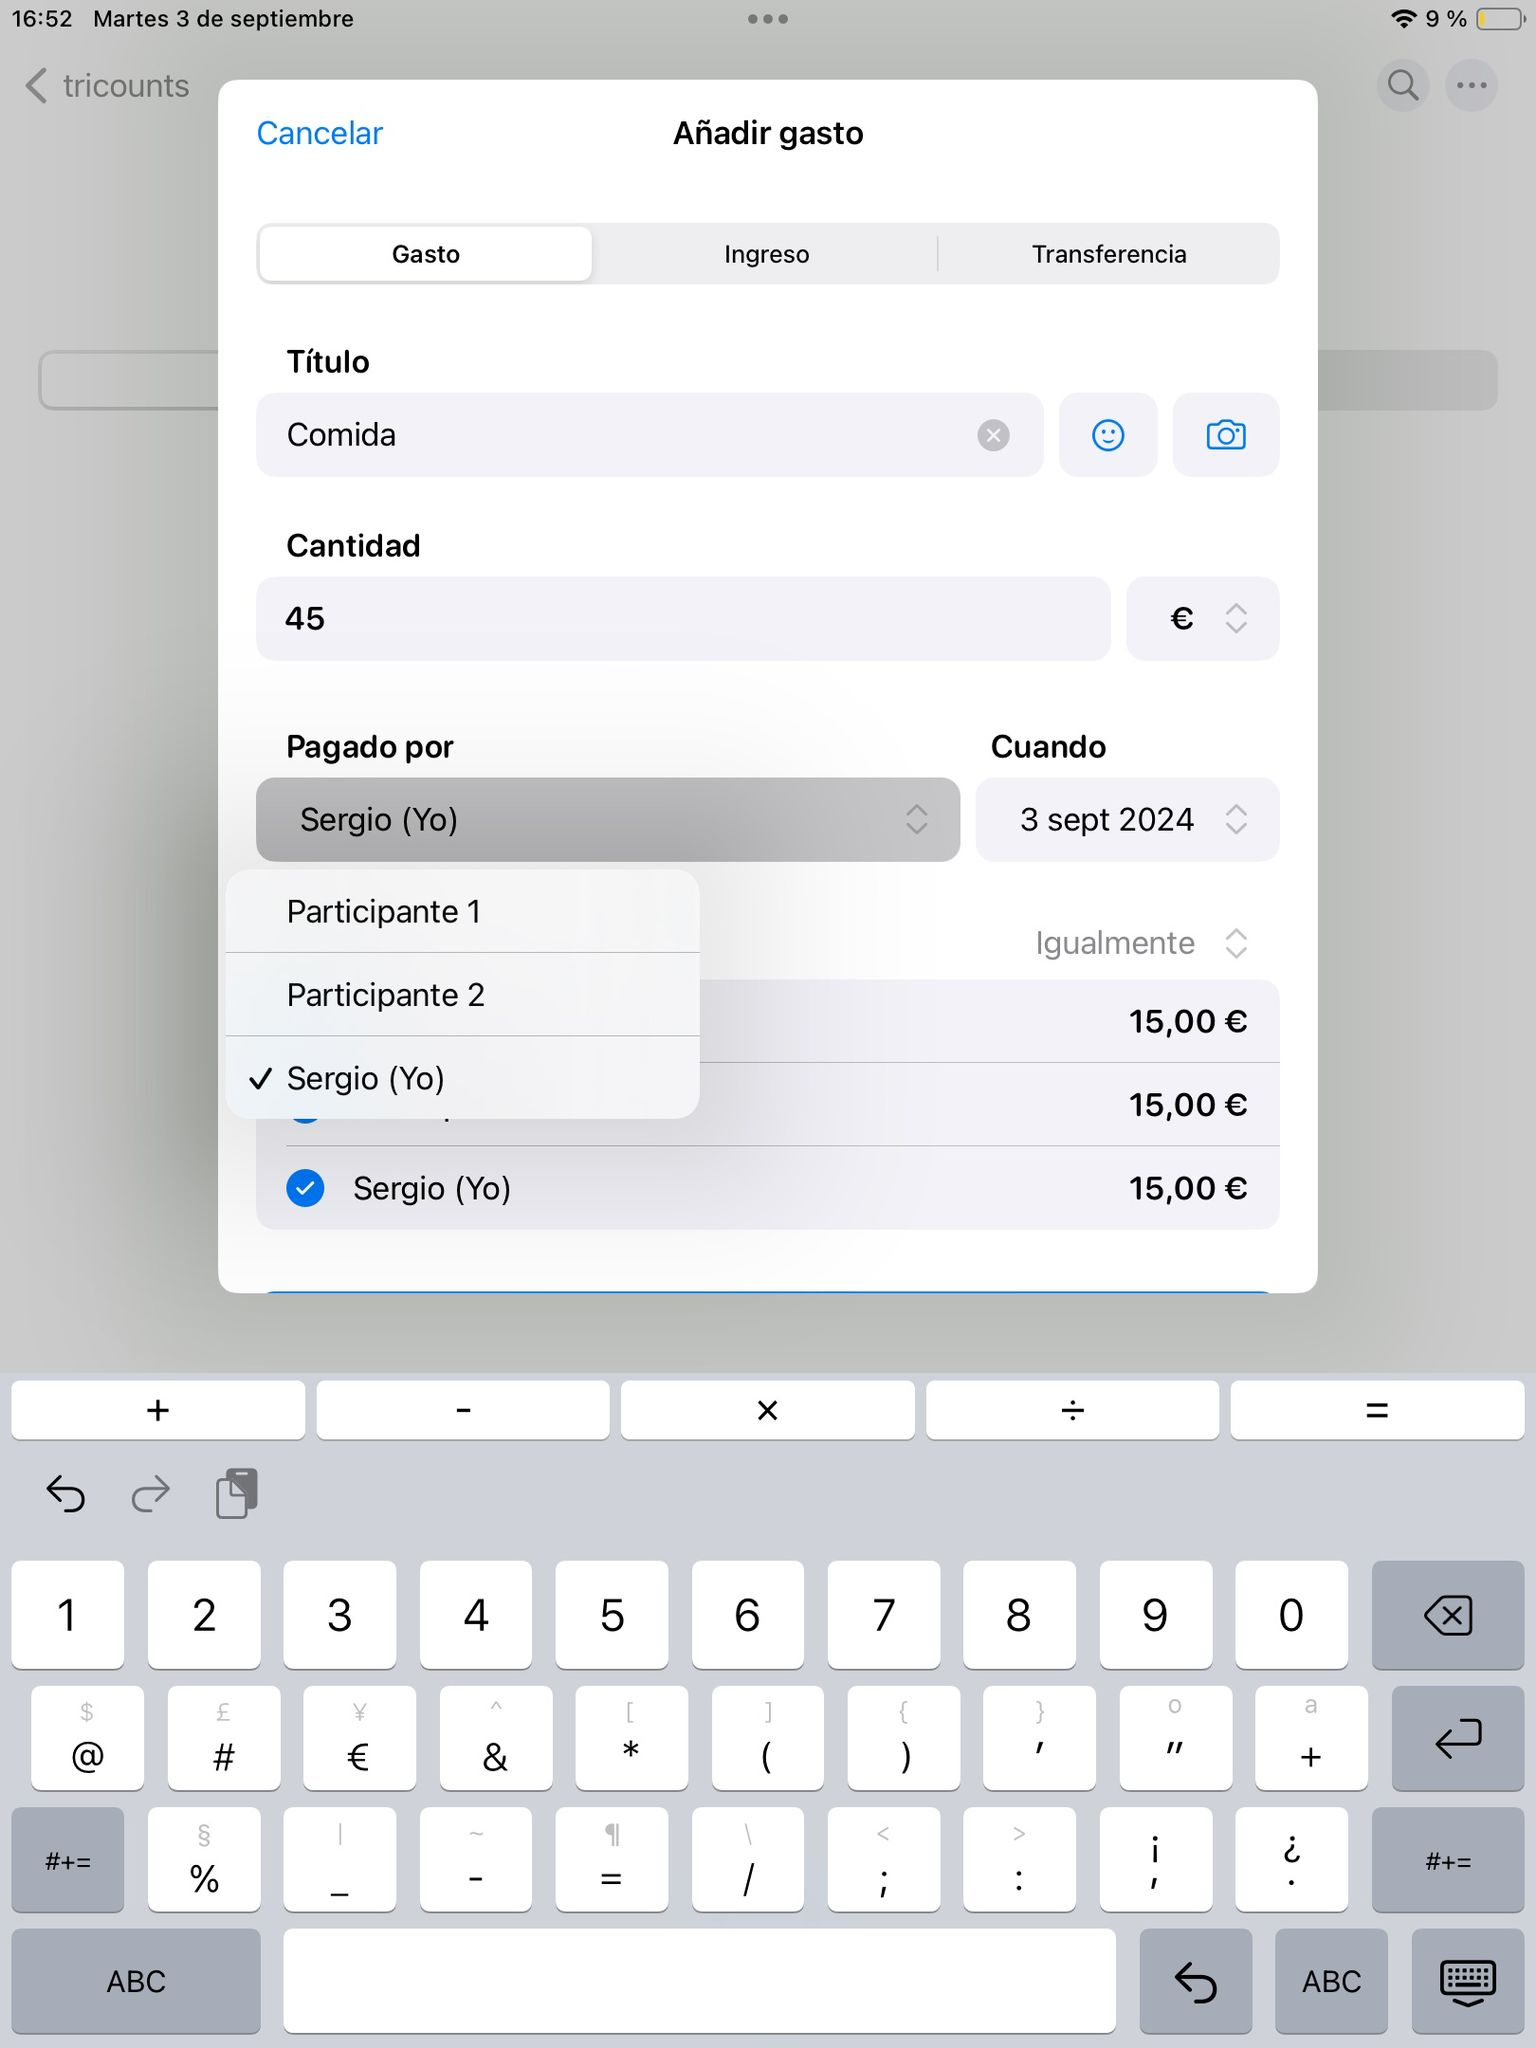
\includegraphics[width=\textwidth]{../capitulos/img/participantes.jpg}
        \caption{Añadir un gasto.}
        \label{participantes}
    \end{minipage}
    \hfill
    \begin{minipage}{0.45\textwidth}
        \centering
        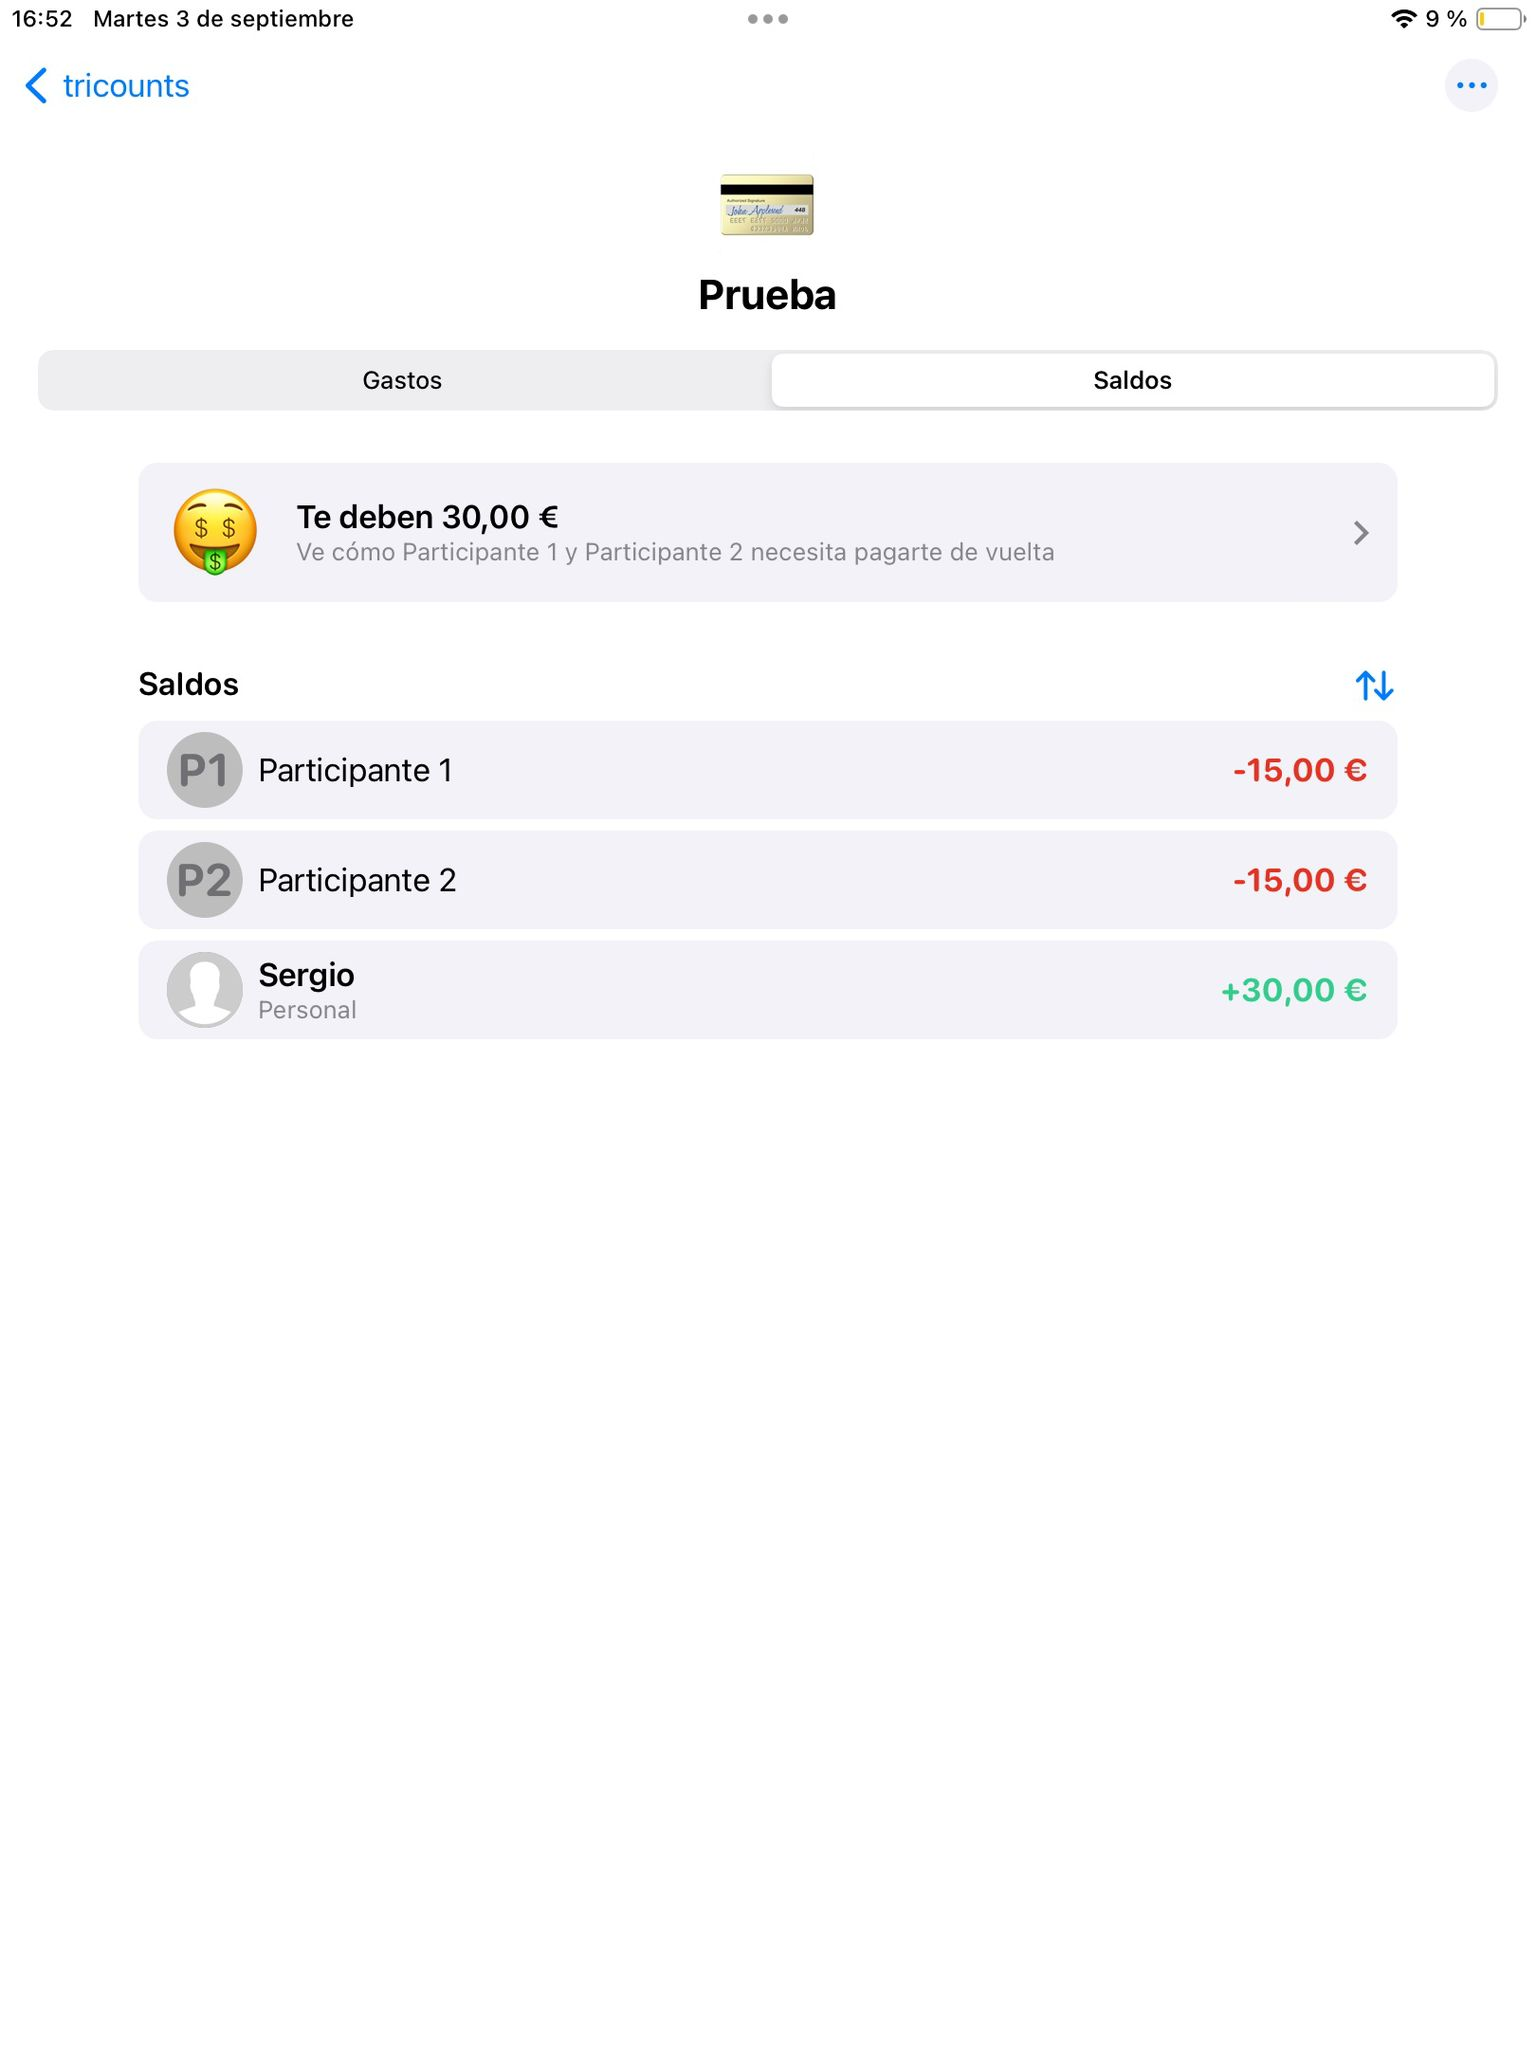
\includegraphics[width=\textwidth]{../capitulos/img/gastos.jpg}
        \caption{Resumen de los gastos y deudas.}
        \label{resumen}
    \end{minipage}
\end{figure}

Con esto ya tendríamos una idea de cómo funciona la aplicación, aunque hay muchas más funcionalidades que se pueden
realizar. 

\subsubsection{Calificación}
\label{subsec:calificacion}
En la tienda oficial de Android (\textit{Google Play}) la aplicación tiene una calificación de 4.8/5 estrellas y cuenta con más de 
10 millones de descargas y en la tienda oficial de Apple (\textit{App Store}) tiene una calificación de 4.7/5 estrellas. La mayoría de comentarios
son positivos y destacan la facilidad de uso y la utilidad de la aplicación.


\subsection{Todoist}
\label{sec:todoist}
Todoist es una aplicación de gestión de tareas y proyectos que ayuda a los usuarios a organizar sus actividades de manera diaria. 
Es ampliamente utilizada tanto por personas como por equipos, debido a su flexibilidad, interfaz intuitiva y capacidad para gestionar
desde simples listas de tareas hasta proyectos complejos. Está disponible para Android, iOS, Windows, Mac y la web.

\subsubsection{Funciones Principales}
\label{subsec:funciones_todoist}

\begin{enumerate}
    \item \textbf{Gestión de Tareas}
    \begin{enumerate}
        \item Añadir Tareas. Pueden crear tareas rápidamente. Cada tarea puede tener un título, una descripción y se puede asignar un proyecto o etiqueta para mantener todo organizado.
        \item Fechas de Vencimiento y Recordatorios. Se puede establecer una fechas límites para las tareas, además de recordatorios específicos, lo que ayuda a asegurarse de que las tareas se hagan a tiempo.
        \item Tareas Recurrentes. Si hay tareas que se repiten, se pueden configurar como tareas recurrentes. 
    \end{enumerate}
    \item \textbf{Proyectos y Subtareas}: 
    \begin{enumerate}
        \item Proyectos. Permite organizar las tareas dentro de proyectos. Los proyectos son carpetas donde se agrupan las tareas relacionadas con un objetivo o área específica.
        \item Subtareas. Para tareas más complejas, pueden descomponerlas en subtareas, permitiendo gestionar pasos más pequeños. 
    \end{enumerate}
    \item \textbf{Etiquetas y Filtros}
    \begin{enumerate}
        \item Etiquetas. Permiten agrupar tareas de diferentes proyectos a través de características comunes-
        \item Filtros. Permite crear vistas personalizadas de las tareas, según criterios como fechas, etiquetas, etc.
    \end{enumerate}
    \item \textbf{Prioridades}. Permite asignar niveles de prioridad a cada tarea, de 1 a 4
    \item \textbf {Colaboración y Gestión de Equipos}
    \begin{enumerate}
        \item Asignar Tareas. En proyectos compartidos, puedes asignar tareas a otros miembros del equipo, facilitando la colaboración en proyectos grupales. 
        \item Comentarios y Archivos. Los usuarios pueden añadir comentarios.
        \item Compartir Proyectos. Puedes compartir proyectos con otros usuarios, lo que permite que todos los miembros vean, añadan o editen tareas dentro de ese proyecto.
    \end{enumerate}
    \item \textbf{Integraciones}. Se integra con una amplia gama de aplicaciones y servicios, como Google Calendar, Slack, Dropbox, etc.
\end{enumerate}

\subsubsection{Modo de Uso}
\label{subsec:uso_todoist}
Lo primero que tenemos que hacer la primera que entramos en la aplicación es registrarnos a través de las diferentes opciones 
que nos permite la aplicación (\textit{Figura \ref{registro}}). Una vez completado este paso nos permite elegir 
el ámbito en el planeas usar la aplicación (he elegido personal porque es la que más se ajusta a la aplicación que estamos buscando).
(\textit{Figura \ref{ambito}}). Hecho todo esto nos lleva a la pantalla principal donde nos muestra las tareas que vencen hoy, en este caso
no aparece ninguna porque aún no hemos añadido nada (\textit{Figura \ref{principal_todoist}}). Si le damos a añadir nos permite poner
una descripción a la tarea, una fecha de vencimiento, una etiqueta, una prioridad, etc. (\textit{Figura \ref{añadir_tarea}}). Una vez añadida
nos aparece la tarea en nuestra lista de tareas pendientes donde la podemos marcar como realiza o no realizada. (\textit{Figura \ref{tarea}}).
También tenemos otra pestaña donde nos muestra un calendario con las tareas que tenemos pendientes por dias, además de la 
tarea que hemos añadido, nos muestra tareas de ejemplo (\textit{Figura \ref{calendario}}). Por último, cabe añadir que la aplicación cuenta
con otra pestaña donde se puede buscar tareas y otra para explorar ya que podemos tener tareas en diferentes bandejas.

\begin{figure}[ht]
    \centering
    \begin{minipage}{0.45\textwidth}
        \centering
        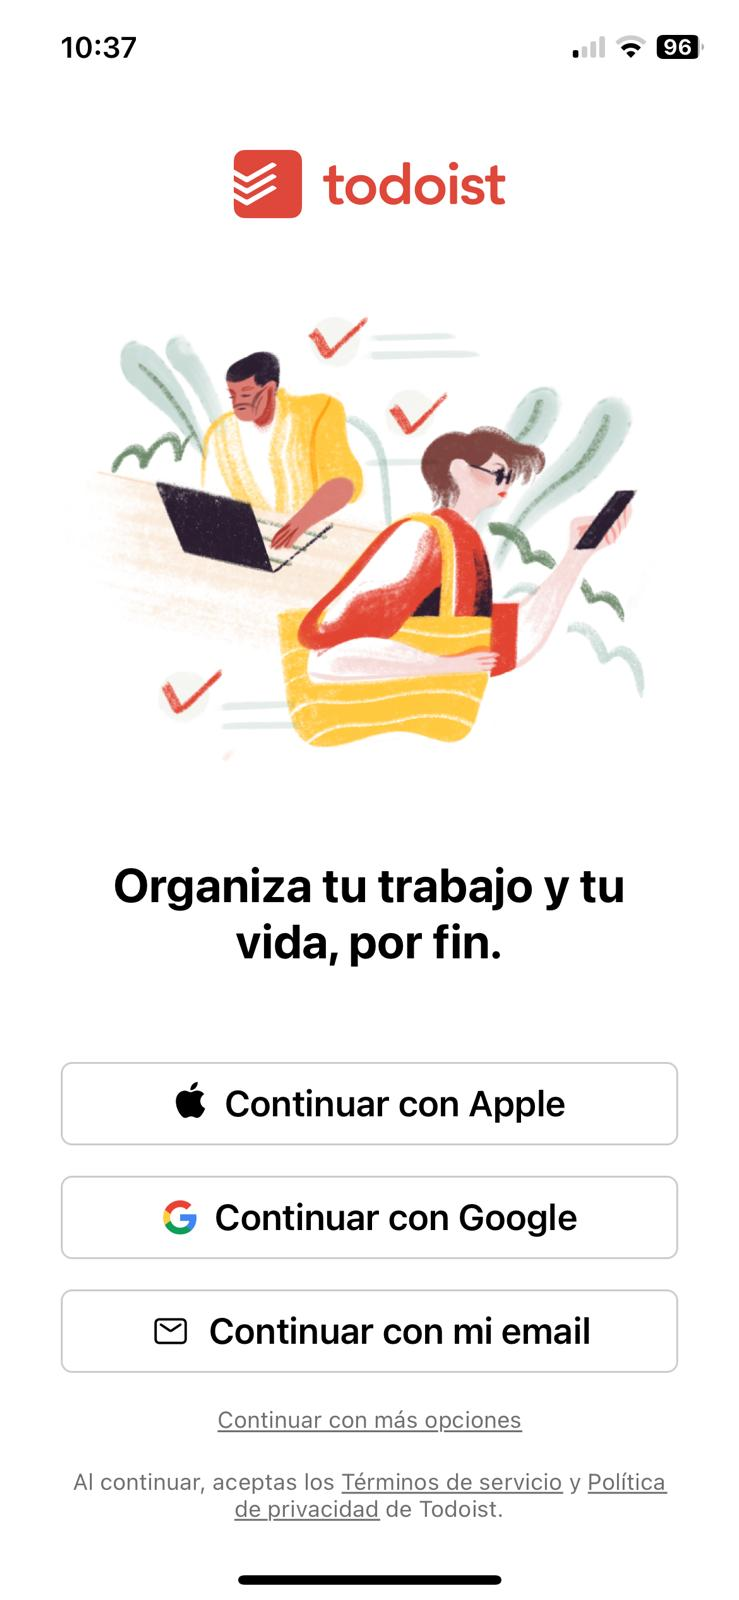
\includegraphics[width=\textwidth]{../capitulos/img/registro_todoist.jpg}
        \caption{Pantalla de registro.}
        \label{registro}
    \end{minipage}
    \hfill
    \begin{minipage}{0.45\textwidth}
        \centering
        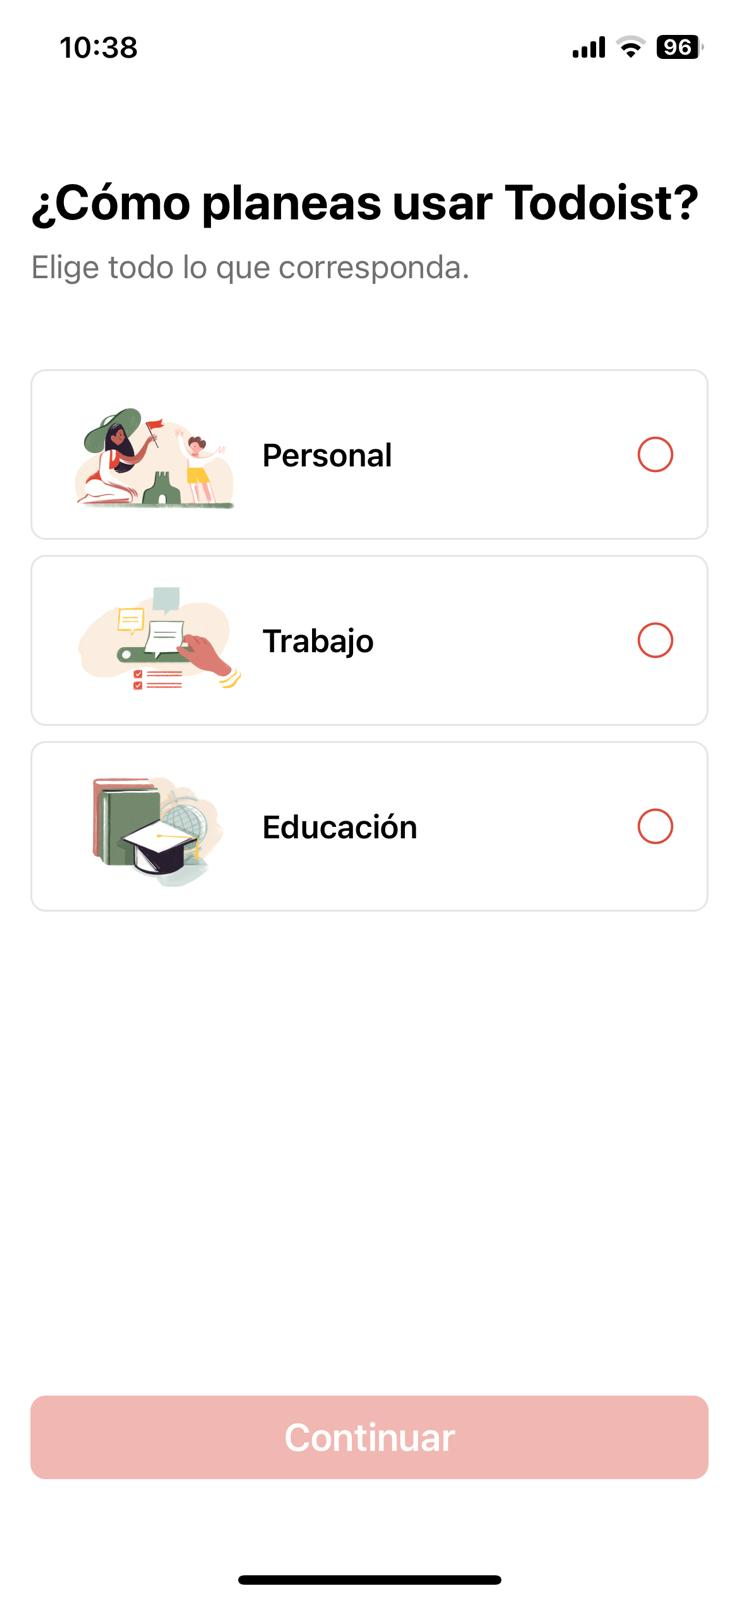
\includegraphics[width=\textwidth]{../capitulos/img/ambito_todoist.jpg}
        \caption{Elegir el ámbito de la aplicación.}
        \label{ambito}
    \end{minipage}
\end{figure}

\begin{figure}[ht]
    \centering
    \begin{minipage}{0.45\textwidth}
        \centering
        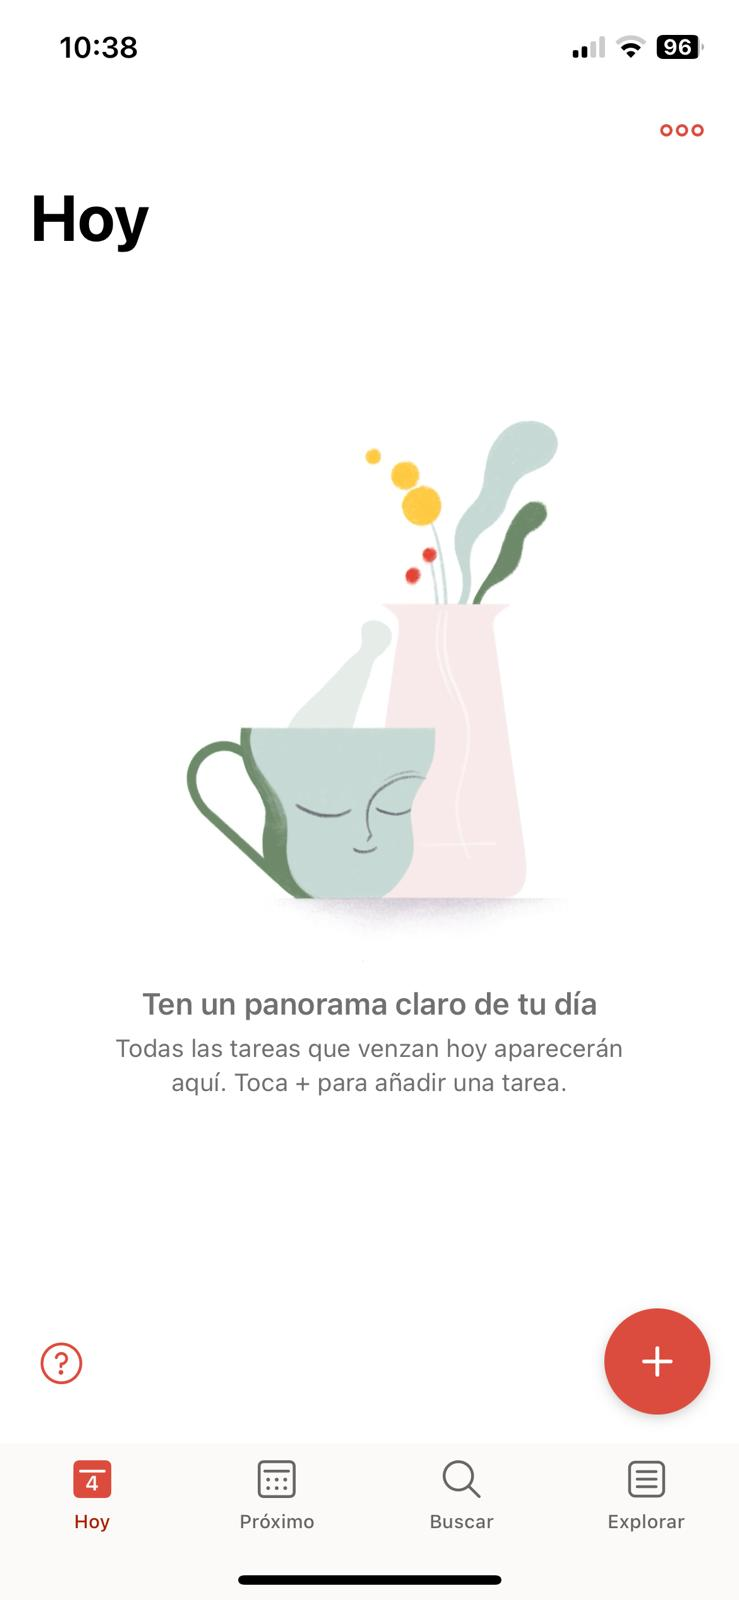
\includegraphics[width=\textwidth]{../capitulos/img/principal_todoist.jpg}
        \caption{Pantalla principal.}
        \label{principal_todoist}
    \end{minipage}
    \hfill
    \begin{minipage}{0.45\textwidth}
        \centering
        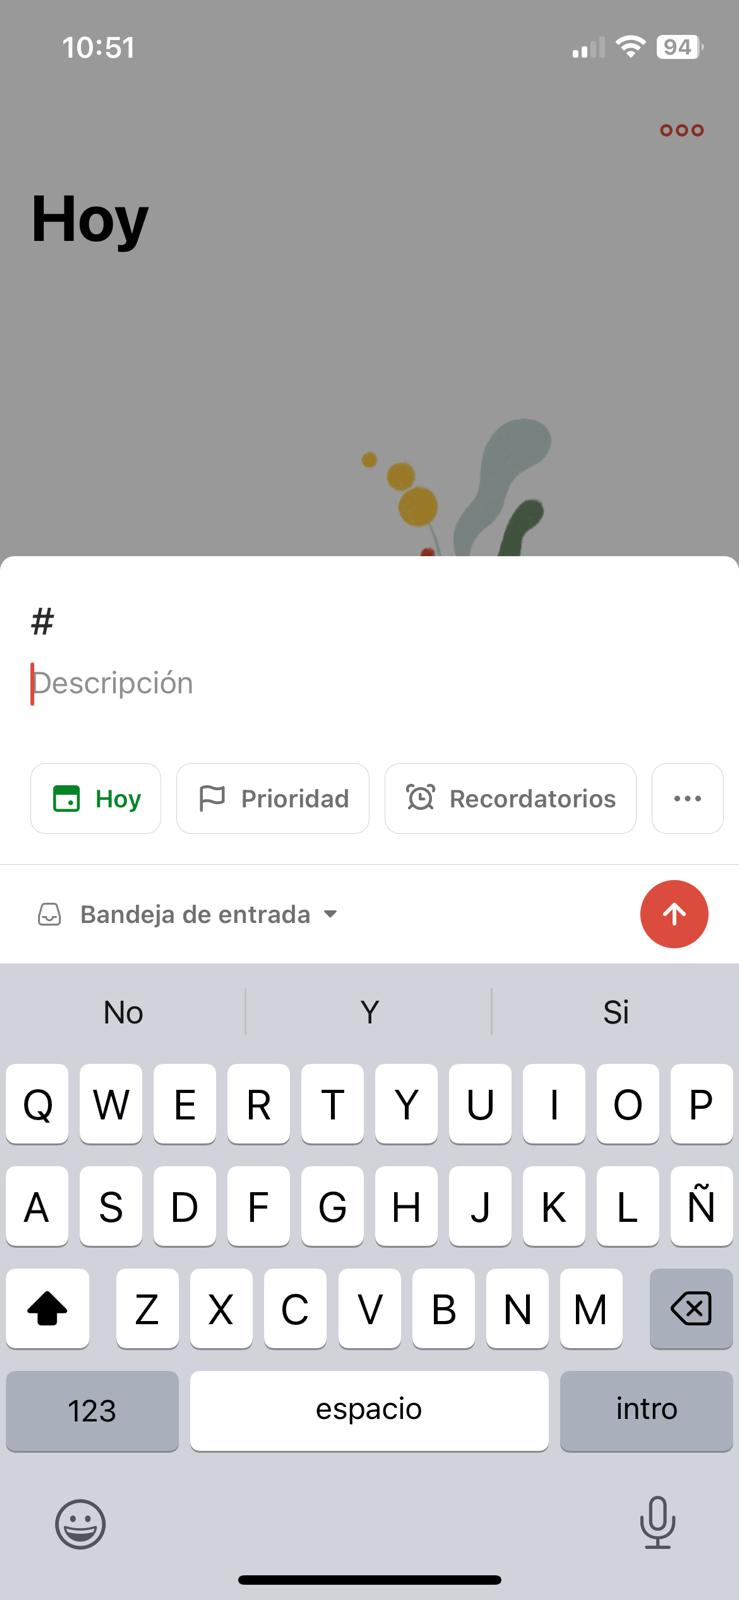
\includegraphics[width=\textwidth]{../capitulos/img/añadir_todoist.jpg}
        \caption{Añadir una tarea.}
        \label{añadir_tarea}
    \end{minipage}
\end{figure}

\begin{figure}[ht]
    \centering
    \begin{minipage}{0.45\textwidth}
        \centering
        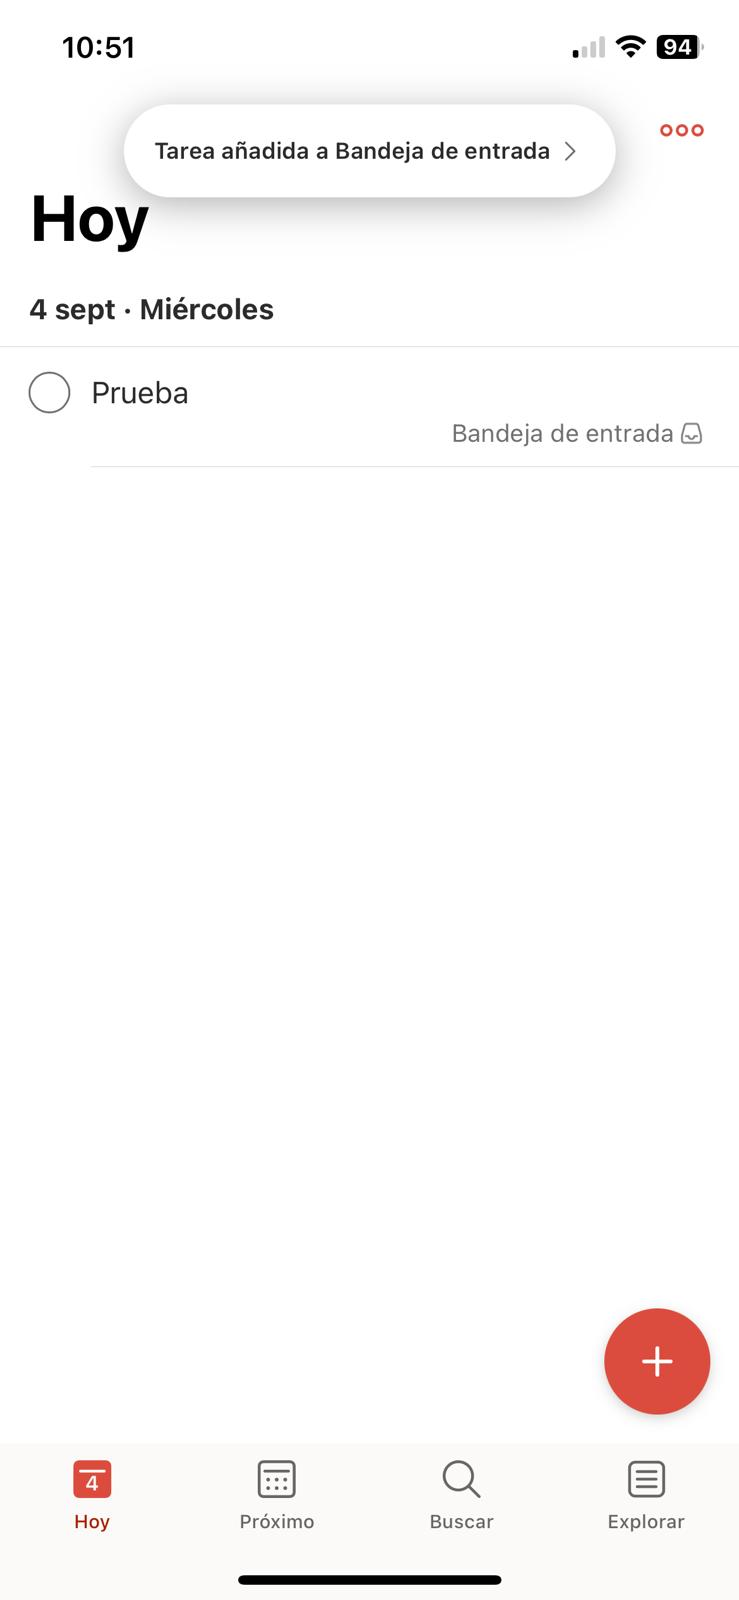
\includegraphics[width=\textwidth]{../capitulos/img/tarea_todoist.jpg}
        \caption{Pantalla con la tarea añadida.}
        \label{tarea}
    \end{minipage}
    \hfill
    \begin{minipage}{0.45\textwidth}
        \centering
        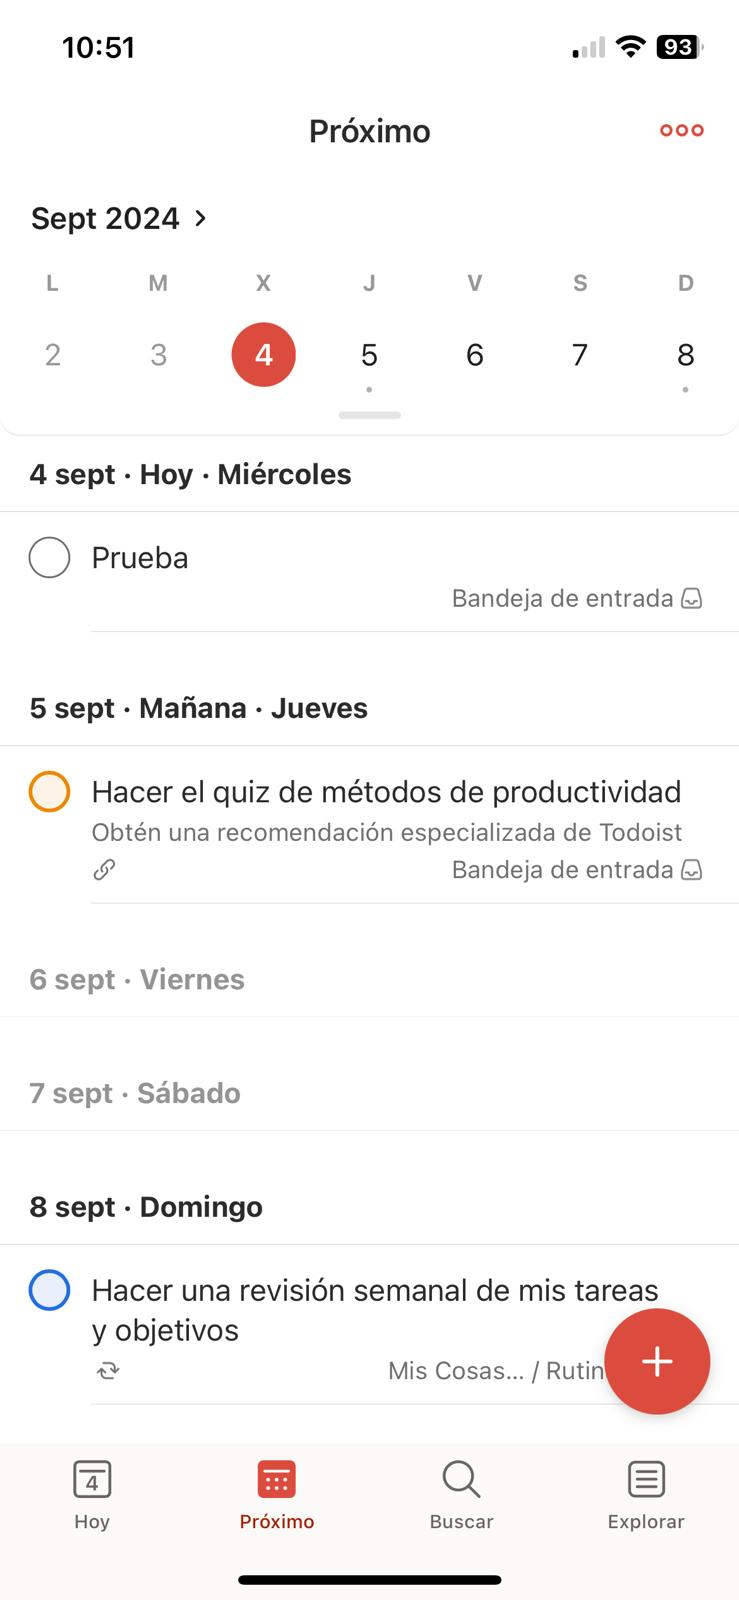
\includegraphics[width=\textwidth]{../capitulos/img/calendario_todoist.jpg}
        \caption{Calendario de tareas.}
        \label{calendario}
    \end{minipage}
\end{figure}

\subsubsection{Calificación}
\label{subsec:calificacion_todoist}
En la tienda oficial de Android (\textit{Google Play}) la aplicación tiene una calificación de 4.5/5 estrellas y cuenta con más de
10 millones de descargas y en la tienda oficial de Apple (\textit{App Store}) tiene una calificación de 4.7/5 estrellas. La mayoría de comentarios
son positivos y destacan la facilidad de uso y la utilidad de la aplicación. La versión de pago tiene un coste de 4.99\texteuro/mes o 47.99\texteuro/año.

\subsection{MeToca}
\label{sec:metoca}
Es una aplicación desarrollada por el gobierno de España con el objetivo de facilitar la organización de tareas del hogar
de manera equitativa y eficiente. Es una iniciativa para promover la corresponsabilidad en el hogar, asegurando que las
responsabilidades domésticas sean distruidas de manera justa entre todos los miembros de la familia. Es gratuita y 
en un principio estaba disponible para Android e iOS, pero en la actualidad solo está disponible para Android.
\subsubsection{Funciones Principales}

\begin{enumerate}
    \item \textbf{Gestión de Tareas del Hogar}
    \begin{enumerate}
        \item Asignación de tareas. Permite asignar tareas a cada miembro del hogar. Las tareas pueden ser de cualquier tipo
        \item Calendario y Recordatorios. Incluye un calendario integrado donde se pueden programar las tareas frecuentes o únicas.
        Además envía recordatorios en caso de no hacerlas a tiempo.
    \end{enumerate}
    \item \textbf{Seguimiento y Cumplimiento}
    \begin{enumerate}
        \item Registro de Tareas Completadas. Cada usuario puede marcar sus tareas completadas y así poder llevar unn control del cumplimiento de responsabilidades.
        \item Estadísticas de Participación. Genera informes y estadísticas sobre cómo se están distribuyendo las tareas y si se están cumpliendo.
    \end{enumerate}
    \item \textbf{Distribución Equitativa}
    \begin{enumerate}
        \item Corresponsabilidad. Fomenta la corresponsabilidad en el hogar a través de la visualización 
        y el seguimiento de tareas todos los miembros pueden ver si las responsabilidades se están distribuyendo de manera equitativa.
    \end{enumerate}
    \item \textbf{Soporte para diferentes tipos de hogares}
    \begin{enumerate}
        \item Adaptabilidad. Está diseñada para ser inclusiva y adapatable para cualquier tipo de hogar o de familia
        \end{enumerate}
\end{enumerate}

\subsubsection{Modo de Uso}
\label{subsec:uso_metoca}
En este caso no he podido probar la aplicación ya que no está disponible para iOS.

\subsubsection{Calificación}
\label{subsec:calificacion_metoca}
En la tienda oficial de Android (\textit{Google Play}) la aplicación tiene una calificación de 1.6/5 estrellas,
con apenas más de 10.000 descargas, aunque los creadores aseguran que tienen muchisimas funcionalidades la mayoría de comentarios
aseguran que no les resulta muy útil.

\subsection{Cozi Family Organizer}
\label{sec:cozi}
Es una aplicación diseñada para ayudar a las familias a organizar y gestionar sus actividades diarias para auidar a las familias a organizar y 
gestionar sus actividades de manera colaborativa. Cozi se enfoca en la simplicidad y en proporcionar funciones esenciales para coordinar 
las actividades de varios miembros de una familia ocupada. Está disponible para Android, iOS y la web. Dispone de una versión 
gratuita que incluye la mayoría de las funcionalidades principales y una versión de pago con funciones adicionales.

\subsubsection{Funciones Principales}
\label{subsec:funciones_cozi}

\begin{enumerate}
    \item \textbf{Calendario Familiar}
    \begin{enumerate}
        \item Calendario Unificado. El calendario de Cozi hace que todos los miembros de la familia tengan acceso a un calendario compartido. 
        Cada miembro de la familia tiene un color asignado, lo que facilita ver quién tiene cada actividad y cuando tiene que hacerla.
        \item Eventos y Recordatorios. Se pueden añadir eventos y establecer recordatorios para asegurar que madie olvide compromisos importantes, cómo
        citas médicas, actividades escolares o eventos familiares.
        \item Notificaciones. La aplicación envía notificaciones a los miembros de la familia sobre los eventos próximos, asegurando que todo estén informados de los planes.
    \end{enumerate}
    \item \textbf{Lista de Compras Compartidas}
    \begin{enumerate}
        \item Lista de Compras Colaborativas. Permite crear y compartir listas de compras entre todos los miembro de la familia, 
        lo que permite que varias personas puedan contribuir a la lista y cualquier miembro puede marcar articulos que ya se han comprado. 
        \item Actualizaciones en Tiempo Real. La lista de compras se actualiza en tiempo real, lo que significa que cualquier cambio que se haga se refleja inmediatamente en todos los dispositivos.
        \item Organización por Tienda. Las listas pueden organizarse por tipo de tienda o categoría.
    \end{enumerate}
    \item \textbf{Listas de Tareas}
    \begin{enumerate}
        \item Tareas Pendientes. Permite crear listas para proyectos domésticos, responsabilidades diarias o cualquier tipo de actividades pendientes
        \item Marcar Completadas. Los usuarios pueden marcarla como hecha, lo que ayuda a mantener un seguimiento claro de lo que se ha logrado
    \end{enumerate}
    \item \textbf{Planificación de Comidas}
    \begin{enumerate}
        \item Organizador de Menús. Facilita organizar las comidas con antelación y evita el estrés diario de decidir qué cocinar. 
        \item Recetas Integradas. Puedes guardar y organizar recetas directamente en la aplicación y con solo un clic. 
        \item Sincronización con el calendario. Los menús planificados pueden sincronizarse con el calendario para que toda la familia lo vea. 
    \end{enumerate}
    \item \textbf{Diario Familiar}. Es una función donde los miembros pueden registrar eventos o recuerdos importantes, como fotos y notas sobre actividades familiares. 
    Además se puede compartir con otro familiares y amigos.
\end{enumerate}

\subsubsection{Modo de Uso}
\label{subsec:uso_cozi}
Después de descargar e instalar esta aplicación, lo primero que nos muestras es una pantalla de registro/inicio de sesión (\textit{Figura \ref{registro_cozi}}).
donde nos pide un nombre, el correo electrónico y una contraseña. Después de crear nuestra cuenta nos muestra una pantalla donde nos pide 
el nombre de nuestra familia y los miembros que la componen (\textit{Figura \ref{familia_cozi}}). Después de esto nos permite añadir un evento al calendario, con
un nombre, la fecha, quién la tiene que realizar, si se repite o no y cúando queremos que nos lo recuerde (\textit{Figura \ref{evento_cozi}}). Una vez completado este 
paso nos muestra el un calendario con todas las tareas que tenemos pendientes (\textit{Figura \ref{calendario_cozi}}). Si nos vamos a la pestaña de "List"
nos muestras todas las listas de compras o de cosas que hacer ya que están divididas en dos pestañas, en la (\textit{Figura \ref{listas}}) podemos ver un ejemplo de lista 
de la compra con un árticulo añadido a una de ellas. Otra de las pestañas que nos ofrece la aplicación es la de "Recetas" donde nos muestra recetas de cocina y además nos deja 
añadir más recetas a través de una url de la receta encontrada (\textit{Figura \ref{recetas}}). Por último, la pestaña final es la de "Familia" donde nos permite configurar información sobre la familia, por ejemplo, 
añadir una foto de perfil o añadir a un miembro más a la familia. 

\begin{figure}[ht]
    \centering
    \begin{minipage}{0.45\textwidth}
        \centering
        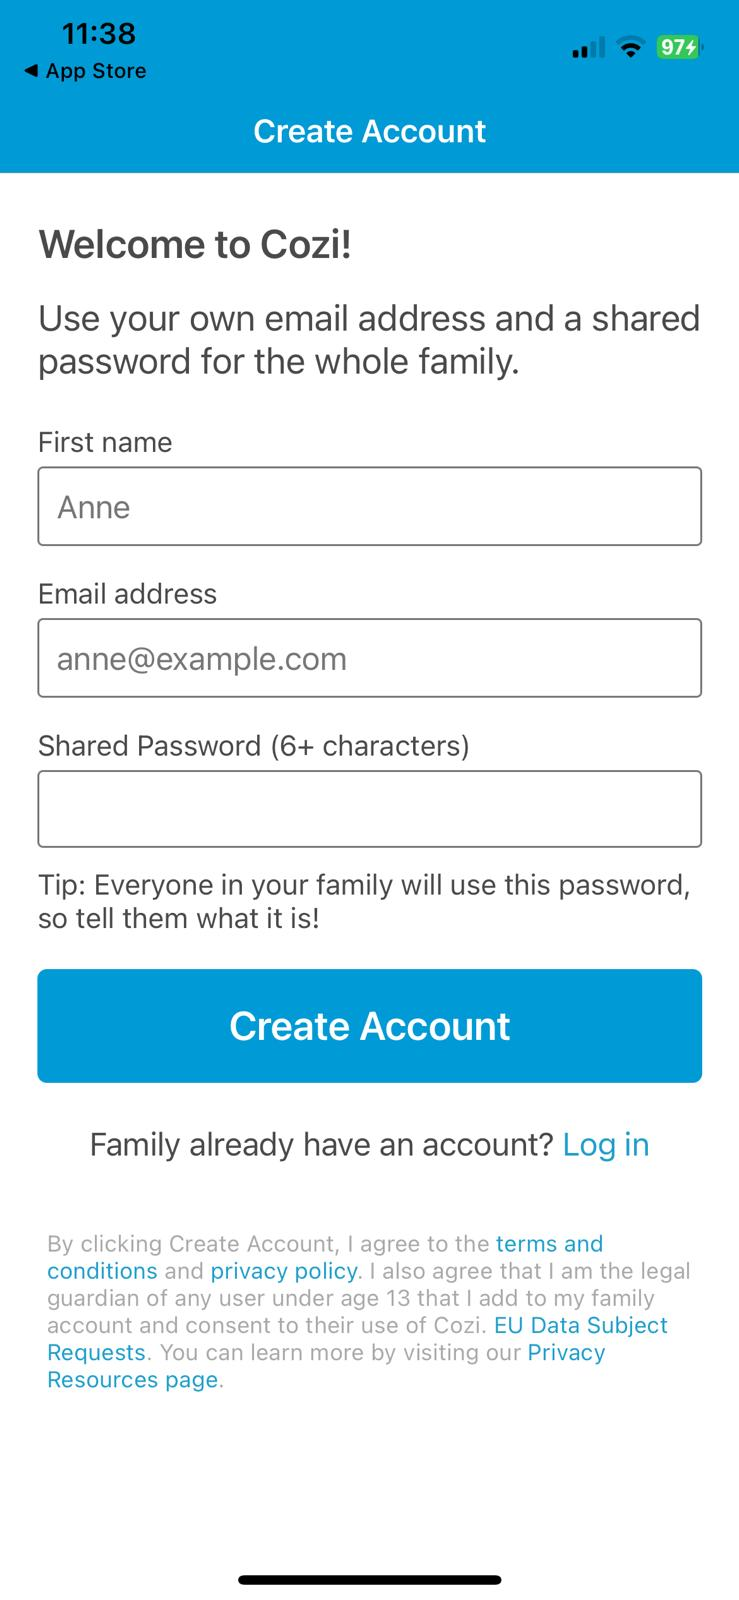
\includegraphics[width=\textwidth]{../capitulos/img/registro_cozi.jpg}
        \caption{Registro.}
        \label{registro_cozi}
    \end{minipage}
    \hfill
    \begin{minipage}{0.45\textwidth}
        \centering
        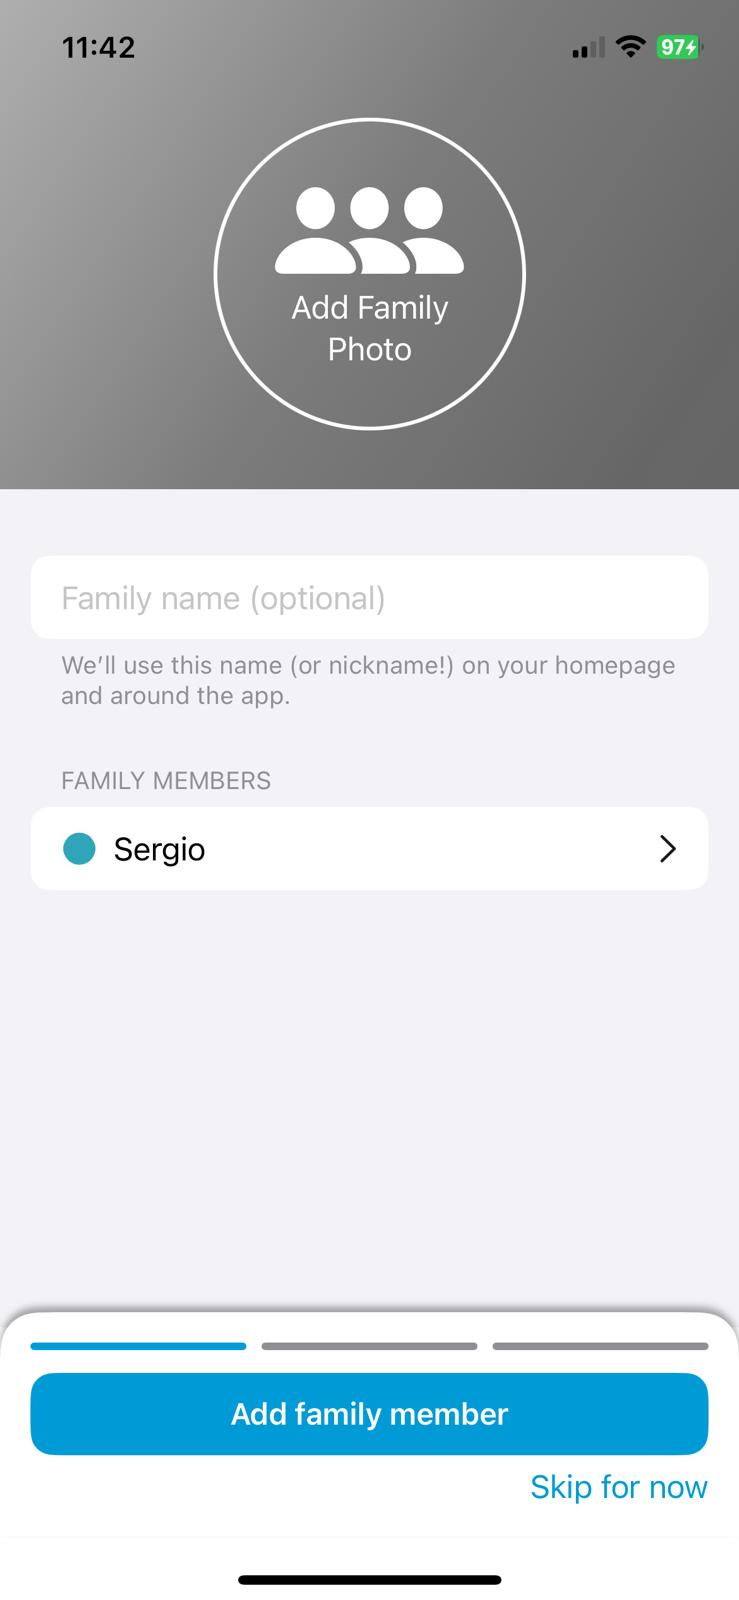
\includegraphics[width=\textwidth]{../capitulos/img/familia_cozi.jpg}
        \caption{Crear una familia.}
        \label{familia_cozi}
    \end{minipage}
\end{figure}

\begin{figure}[ht]

    \begin{minipage}{0.45\textwidth}
        \centering
        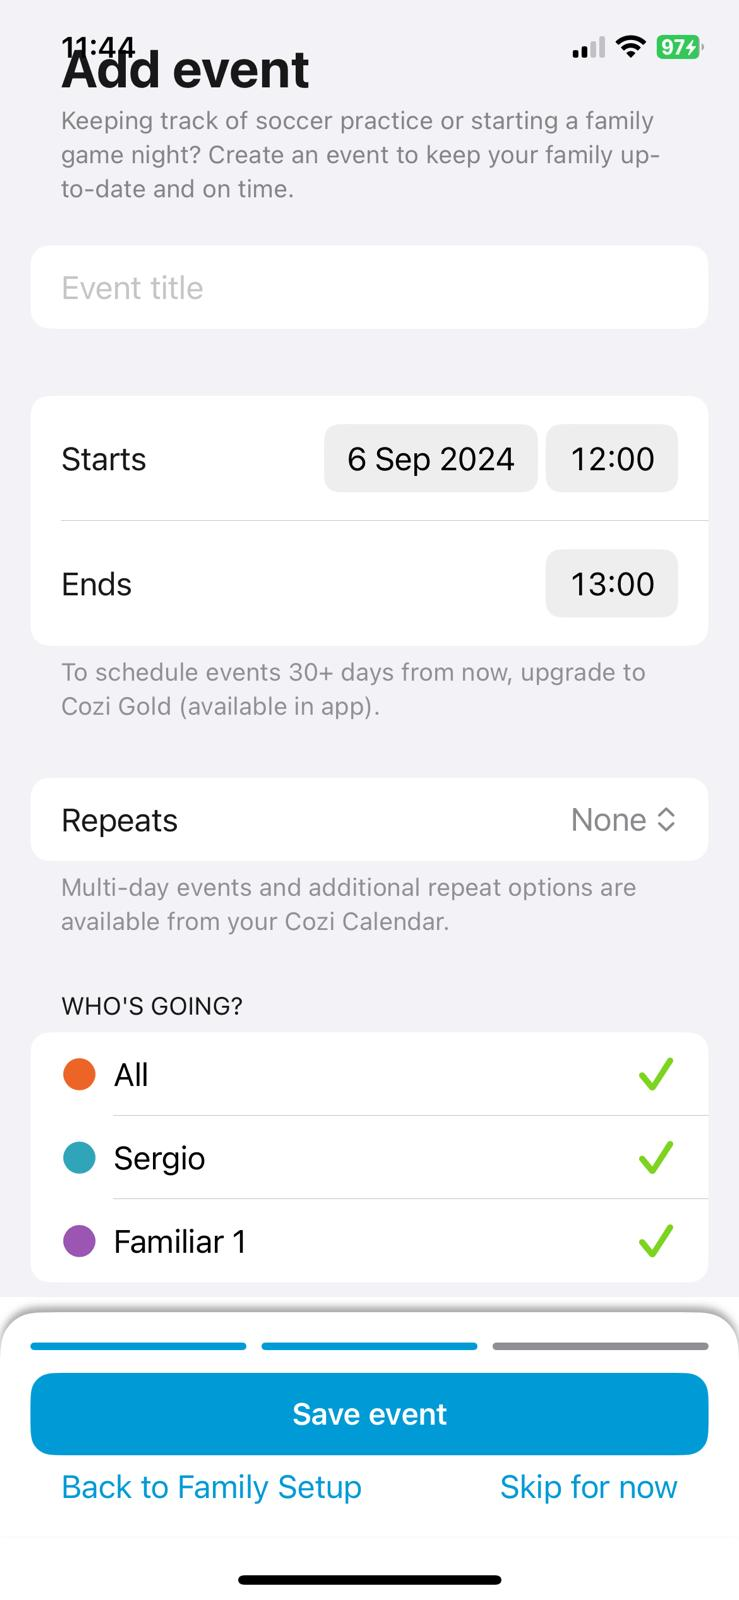
\includegraphics[width=\textwidth]{../capitulos/img/evento_cozi.jpg}
        \caption{Añadir un evento.}
        \label{evento_cozi}
    \end{minipage}
    \hfill
    \begin{minipage}{0.45\textwidth}
        \centering
        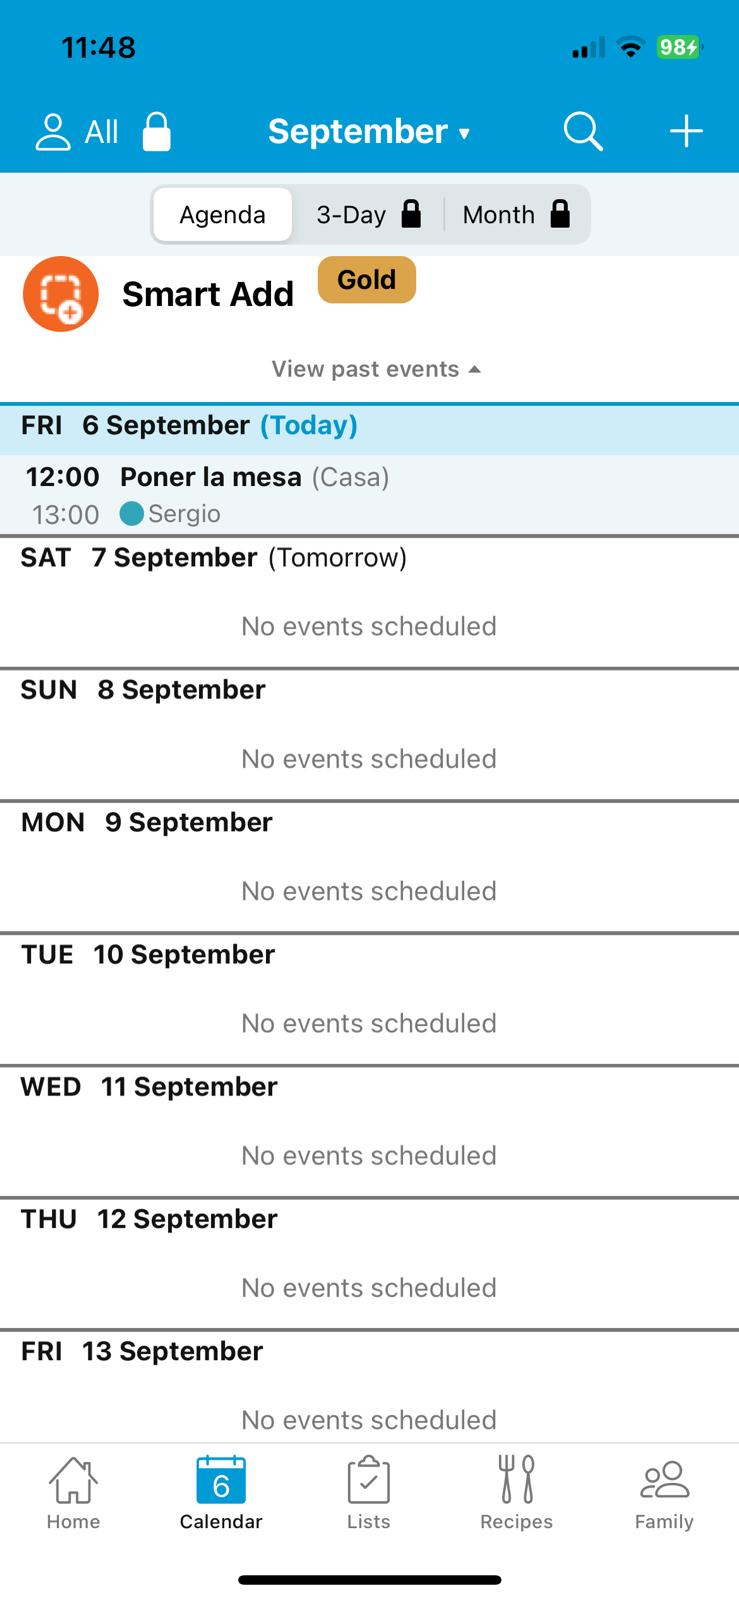
\includegraphics[width=\textwidth]{../capitulos/img/calendario_cozi.jpg}
        \caption{Calendario.}
        \label{calendario_cozi}
    \end{minipage}
\end{figure}

\begin{figure}[ht]

    \begin{minipage}{0.45\textwidth}
        \centering
        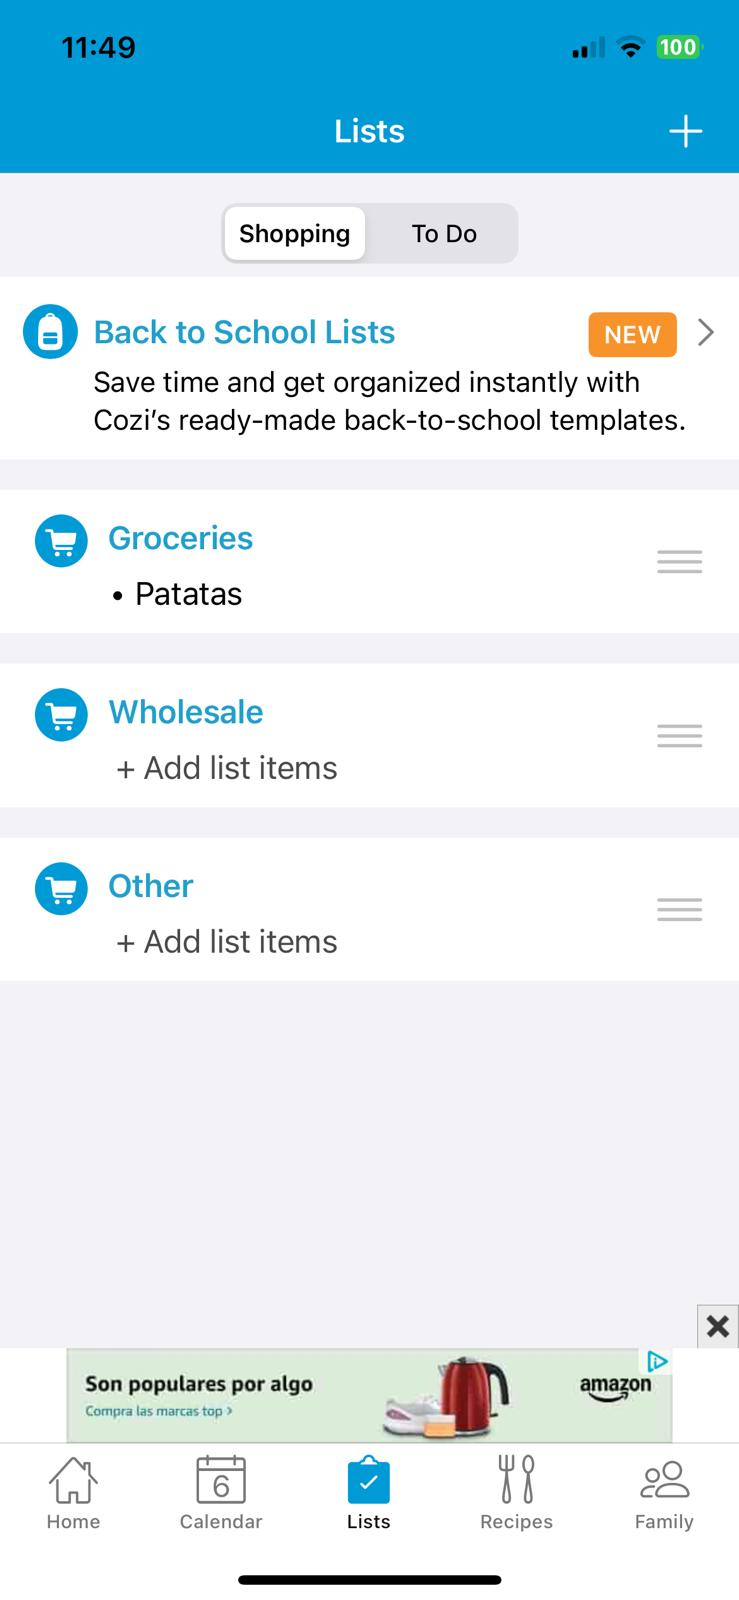
\includegraphics[width=\textwidth]{../capitulos/img/listas_cozi.jpg}
        \caption{Listas de la compra.}
        \label{listas}
    \end{minipage}
    \hfill
    \begin{minipage}{0.45\textwidth}
        \centering
        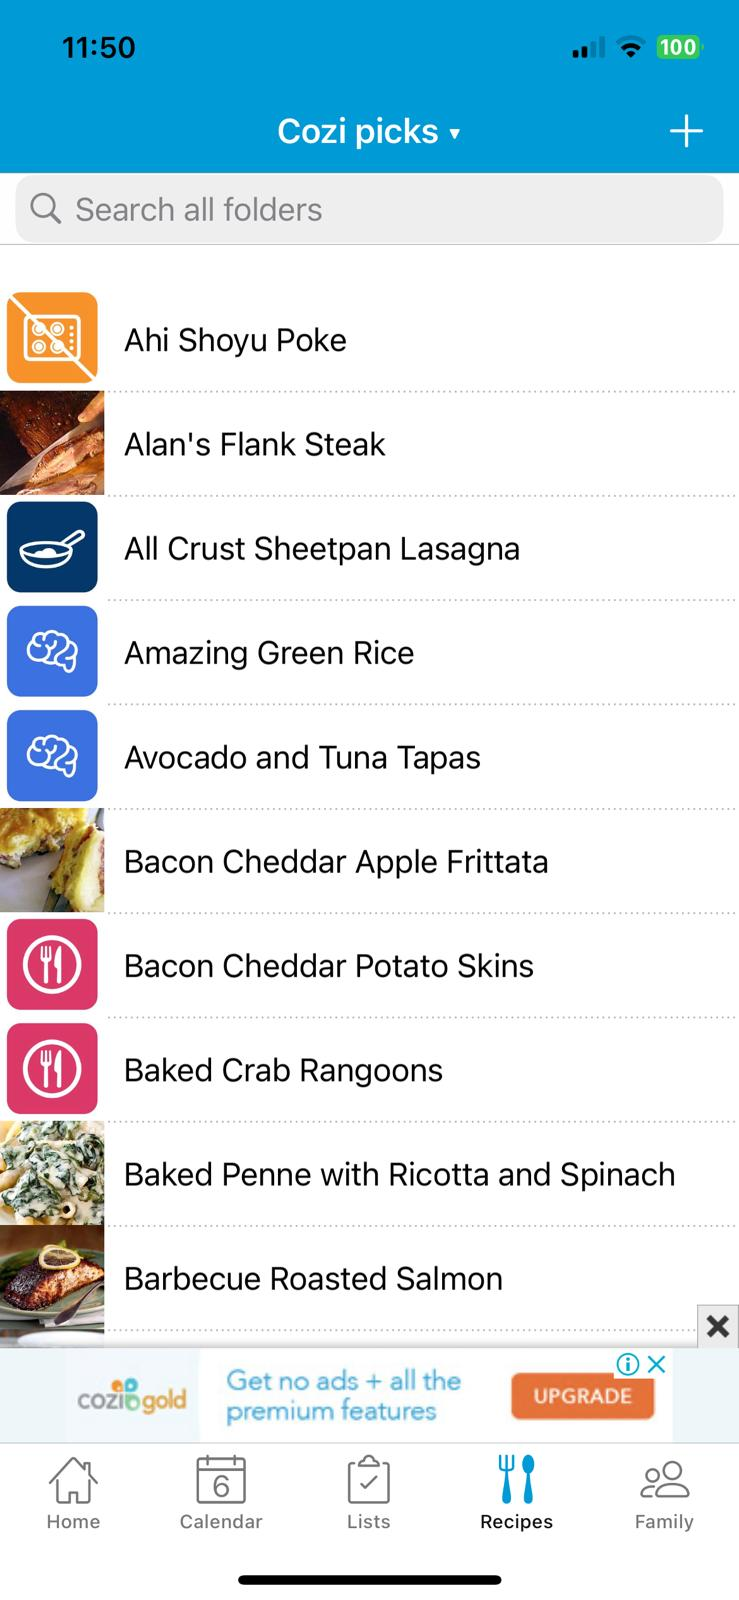
\includegraphics[width=\textwidth]{../capitulos/img/recetas_cozi.jpg}
        \caption{Recetas.}
        \label{recetas}
    \end{minipage}
\end{figure}




\subsubsection{Calificación}
\label{subsec:calificacion_cozi}
En la tienda oficial de Android (\textit{Google Play}) la aplicación tiene una calificación de 4.1/5 estrellas y cuenta con más de 5 millones de descargar. 
En la tienda oficial de Apple (\textit{App Store}) tiene una calificación de 4.8/5 estrellas. La mayoría de comentarios son positivos y destacan la facilidad de uso y la utilidad de la aplicación.
Por lo que he podido observar la página esta completamente en inglés. 

\subsection{OurHome}
\label{sec:ourhome}
Es una aplicación que ayuda a familias a organizar y gestionar tareas, compras y responsabilidades diarias de manera colaborativa. 
Está diseñada para facilitar la administración de tareas en el hogar y fomentar la cooperación familiar mediante asignación de tareas, 
el seguimiento de recompensas y la planificación de compras. 

\subsubsection{Funciones Principales}
\label{subsec:funciones_ourhome}

\begin{enumerate}
    \item  \textbf{Asignación de Tareas}. Permite asignar y crear tareas a los miembros de la familia, definiendo la frecuencia y quien debe hacer cada tarea y en qué plazo.
    Además incluye un sistema de recompensas basado en puntos, donde los miembros ganan puntos al completar tareas.
    \item \textbf{Lista de Compra Compartida}. Incluye una lista de compras integrada que puede ser gestionada por cualquier miembro de la familia. Permite categorizar artículos y marcarlos como comprados.
    \item \textbf{Calendario Familiar}. Incluye un calendario compartido donde se pueden añadir eventos y recordatorios, donde cada miembro puede ver y agregar eventos.
    \item \textbf{Seguimiento de Objetivos}. Permite a los padres establecer objetivos específicos para los niños o cualquier miembro de la familia, cómo hábitos de estudio o rutinas diarias 
    \item \textbf{Sistema de notificaciones}. Los usuarios reciben notificaciones cuando se les asigna una tarea, se acerca la fecha límite o se actualiza la lista de compras.
\end{enumerate}

\subsubsection{Modo de Uso}
\label{subsec:uso_ourhome}
Si nos metemos desde la página web oficial de la aplicación, nos aparece un enlace para que la descarguemos en nuestro dispositivo iOS, 
sin embargo, en mi dispositivo iOS no me da la opción de instalarmela, por lo tanto, tras investigar, llegué a la conclusión de que la aplicación no 
está disponible para nuestra región.

\subsubsection{Calificación}
\label{subsec:calificacion_ourhome}
En la tienda oficial de Android (\textit{Google Play}) la aplicación tiene no tiene ningún tipo de calificación y solo cuanta con un poco más de 500 descargas. 
No aparece ningún tipo de comentario por lo tanto se deduce, que no es una aplicación muy popular. 


\subsection{Comparativa}
\label{sec:comparativa}

A continuación se muestra una tabla comparativa de las aplicaciones analizadas, donde se resumen las principales características y funcionalidades de cada una: 

\begin{table}[ht]
    \centering
    \resizebox{\textwidth}{!}{%
    \begin{tabular}{|c|c|c|c|c|c|}
        \hline
        & \textbf{Tricount} & \textbf{Todoist} & \textbf{MeToca} & \textbf{Cozi Family Organizer} & \textbf{OurHome} \\ \hline
        Plataforma & Android, iOS y web & Android, iOS, Windows, Mac y web & Android & Android, iOS y web & Android \\ \hline
        Coste & Grautito & Grautito y Pago & Gratuito & Grautuito y Pago & Gratuito \\ \hline
        Calificación Media  & 4.75 & 4.6 & 1.6  & 4,45 & -- \\ \hline
        Control de Gastos & \checkmark & -- & -- & -- & -- \\ \hline
        Gestión de Tareas & -- & \checkmark & \checkmark & \checkmark & \checkmark \\ \hline
        Calendario & -- & \checkmark & -- & \checkmark & \checkmark \\ \hline
        Lista de Compras & -- & -- & -- & \checkmark & \checkmark \\ \hline
        Asignación de Tareas & -- & -- & \checkmark & \checkmark & \checkmark \\ \hline
        
      
    \end{tabular} %
    }

\end{table}

\newpage

\section{Estudio de la distribución del tiempo y gestión del hogar en entornos compartidos}

Un estudio del \textit{American Time Use Survey (ATUS)}, analiza la distribución del tiempo que las personas dedican a la administración del hogar
y cómo esta tarea se realiza en intervalos dispersos. Este estudio revela patrones en las actividades domésticas y ayuda a entender los 
desafío de coordinación y planificación en hogares donde las responsabilidades se dividen entre varias personas. El estudio muestra
que las tareas del hogar, como la limpieza, la preparación de comidas, la organización y la gestión de finanzas, tienden a realizarse en 
intervalos de tiempo que varían significativamente entre los distintos miembros del hogar. Esto es problemático en hogares compartidos, como 
los estudiantes o trabajadores, donde la disponibilidad de cada persona depende de su carga académica o laboral. La falta de tiempos fijos y 
la irregularidad en la dedicación a las tareas puede generar problemas de coordinación, ya que cada miembro tiene su propio horario, lo que impide
una rutina doméstica unificada.

Otro hallazgo importante de este estudio es que las tareas domésticas se realizan de manera inconsistente debido a limitaciones de tiempo y energía, especialmente
entre aquellos con empleos de tiempo completo o estudiante con cargas académicas pesadas. Esta incosistencia es común en los hogares compartidos,
donde la carga se divide entre varias personas sin un sistema claro de asignación de responsabilidades o seguimiento. Sin herramientas adecuadas
para la organización, es posible que algunas tareas queden sin realizar o que recaigan siempre en las mismas personas, generando frustración y posibles 
conflictos.

El estudio también resalta que, a medida que los individuos se ven cada vez más presionados por sus estudios o trabajos, tienden a posponer las tareas del hogar, lo cual se 
agrava en entornos de convivencia compartida. Este aplazamiento puede llevar a una acumulación de tareas, que a su vez aumenta el nivel de estrés de los residentes y genera tensiones en el hogar.

Por último, los resultados también sugieren que la organización efectiva del hogar es crucial para el bienestar de sus miembros. En el contexto de hogares compartidos,
el uso de herramientas de planificación o aplicaciones específicas podría mejorar significativamente la administración de tareas y reducir el 
estrés relacionado con el hogar \cite{american2022}.





\section{Estudio sobre los desafíos financieros en viviendas estudiantiles compartidas}
El estudio basado en datos de HUD, examina los desafíos financieros que enfrentan los estudiantes en viviendas compartidas. Uno de los hallazgos
principales de este estudio es que los contratos de arrendamiento de las viviendas a menudo requieren compromisos anuales. Los estudiantes deben 
seguir pagando el alquiler durante todo el año, incluso en períodos en que la vivienda está vacía, como los meses de verano. Este requisito genera una carga
financiera adicional, ya que los estudiantes deben encontrar formas de cubrir los pagos durante esos meses.

También señala que la organización de los gastos compartidos es una tarea compleja para los estudiantes. Dado que los contratos incluyen puede incluir 
diferentes servicios, la variación en las facturas mensuales añade dificultad al reparto equitativo de costes. Muchos estudiantes carecen de herramientas 
y sistemas de organización, lo que provoca confusión y conflictos en cuanto a las cantidades que cada miembro debe pagar. Esto puede ser 
díficil de gestionar cuando uno o varios de los residentes enfrentan problemas financieros, ya que retrasos o impagos afectan a todos los miembros del hogar.

Por último, este estudio también examina cómo las dificultades para gestionar los gastos afectan no solo la situación financiera de los estudiantes, 
sino también su bienestar general y rendimiento académico. La preocupación por la estabilidad financiera y la tensión asociada con la administración de los 
costos compartidos afectan a los estudiantes a nivel psicológico y académico, ya que deben dedicar su tiempo y energía a resolver estos problemas, lo que limita 
su concentración en los estudios. \cite{hud2022}

\newpage

\section{Legislación actual de protección de datos}

La \textbf{Ley de Protección de Datos} está diseñada para garantizar el derecho a la privacidad y 
la protección de los datos personales, evitando el uso indebido o la divulgación de la información 
personal de personas. En la Unión Europea, la normativa más relevante es el 
\textbf{Reglamento General de Protección de Datos (GDPR)}, que entró en vigor en 2018 y 
establece un estándar estricto para el manejo de datos en todos los países miembros, aplicando también 
a empresas fuera de la UE que traten datos de ciudadanos europeos. En España, esta ley se complementa con 
la \textbf{Ley Orgánica de Protección de Datos y Garantía de los Derechos Digitales (LOPD-GDD)}, que adapta
el GDPR pero al contexto español.

Las principales medidas de este reglamento son:
\begin{enumerate}
    \item \textbf{Consentimiento explícito:} Las organizaciones deben obtener el consentimiento explícito de los usuarios antes de recopilar sus datos. Este consentimiento debe ser claro, específico e informado, lo que significa que los usuarios deben saber exactamente qué datos se recogen y para qué fines se usarán.
    \item \textbf{Derecho al Acceso, Rectificación y Supresión:} Los usuarios tienen el derecho de acceder a sus datos personales, solicitar correciones o eliminarlos. Esto se conoce como \textit{derecho al olvido} y permite a los usuarios mantener control sobre su información en línea.
    \item \textbf{Transparencia y Finalidad:} Los empresas deben informar a los usuarios sobre qué datos recopilan, el propósito de dicha recopilación y durante cuánto tiempo los conservarán. Esto busca evitar el almacenamiento de excesivo de datos y el uso para fines distintos a los incialmente indicados.
    \item \textbf{Seguridad de los datos:} Las organizaciones deben implementar medidas de seguridad para proteger los datos, como el cifrado y las políticas de acceso restringido. Estas medidas están orientadas a minimizar el riesgo de filtraciones de datos y accesos no autorizados.
    \item \textbf{Notificación de brechas de seguridad:} Si ocurre una violación de seguridad que afecte datos personales, las empresas deben notificar a las autoridades competentes y a los afectados en un plazo de 72 horas, asegurando así una respuesta rápida que mitigue posibles daños.
\end{enumerate}

Estas medidas buscan proteger los derechos de privacidad de los usuarios y obligan a las empresas a adoptar prácticas de manejo de datos que respeten la seguridad, confidencialidad y transparencia.


\newpage

\section{Estudio de usabilidad y accesibilidad}
\subsection{Estudio de usabilidad}
La \textbf{usabilidad} se refiere a la facilidad con la que los usuarios pueden interactuar con un producto o sistema para alcanzar sus 
objetivos de manera efectiva, eficiente y satisfactoria. Según la norma ISO/IEC 9241-11, la usabilidad se define como "la eficacia, eficiencia y satisfacción 
con la que un producto permite alcanzar objetivos específicos a usuario específicos en un contexto de uso específico". \cite{wikipedia2025}

Las principales características de la usabilidad son: 
\begin{enumerate}
    \item \textbf{Facilidad de aprendizaje:} Capacidad del sistema para permitir que nuevos usuarios realicen tareas básicas la primera vez que lo utilizan. \cite{coursera2023}
    \item \textbf{Eficiencia:} Una vez que los usuarios han aprendido el diseño, deben poder realizar tareas con rapidez y precisión. \cite{coursera2023}
    \item \textbf{Memorabilidad:} Los usuarios deben poder retomar el uso del sistema después de un período de inactividad sin necesidad de reaprender todo. \cite{coursera2023}
    \item \textbf{Manejo de errores:} El sistema debe minimizar la frecuencia y gravedad de los errores, y permitir una recuperación fácil cuando ocurran. \cite{coursera2023}
    \item \textbf{Satisfacción:} El uso del sistema debe de ser agradable, proporcinando una experiencia positiva al usuario \cite{coursera2023} 
\end{enumerate}

La usabilidad es fundamental para garantizar que los productos o sistemas sean accesibles y efectivos para los usuarios previstos. Un alto nivel de usabilidad
conduce a una mayor satisfacción del usuario, reduce los errores y aumenta la eficiencia en la realización de tareas. Además, mejora la adopción del producto 
y puede proporcionar una ventaja competitiva en el mercado. Una buena usabilidad asegura que los usuarios puedan navegar e interactuar con el sistema de manera intuitiva, encontrando 
la información que buscan y completando acciones sin dificultades. \cite{adverthia2019}

\subsection{Estudio de accesibilidad}
La \textbf{accesibilidad} en el desarrollo de software se refiere al diseño de aplicaciones que pueden ser utilizadas por el mayor número de 
personas posibles, incluyendo aquellas con discapacides físicas, cognitivas o sensoriales. Según la documentación de Microsoft, diseñar software 
accesible implica garantizar que los programas y sus funcionalidades estén disponibles para una amplia gama de usuarios, independientemente de sus capacidades \cite{microsoft2023}.

Las principales características de la accesibilidad son: 

\begin{enumerate}
    \item \textbf{Perceptible:} La información y los componentes de la interfaz deben ser presentados de manera que los usuarios pueden percibirlos. Esto incluye proporcionar alternativas textuales para contenido no textual 
    y asegurar que el contenido sea adaptable a diferentes formatos \cite{torresburriel2024}
    \item \textbf{Operable:} Los componentes de la interfaz y la navegación deben ser utilizables por todos los usuarios. Por ejemplo, garantizar que todas las funciones sean accesibles mediante teclado y proporcionar suficiente tiempo para que los 
    usuarios realicen tareas \cite{torresburriel2024}
    \item \textbf{Comprensible:} La información y el funcionamiento de la interfazz deben ser claros y coherentes, facilitando la comprensión y el uso del sistema. Esto implica utilizar un lenguaje sencillo y predecible, así como proporcionar asistencia cuando sea necesario \cite{torresburriel2024}
    \item \textbf{Robusto:} El contenido debe ser lo suficientemente robusto como para ser interpretado de manera fiable por una amplia de agentes de usuario, incluyendo tecnologías de asistencia. Esto asegura que el contenido siga siendo accesible a medida que las tecnlogías avanzan. \cite{torresburriel2024}
\end{enumerate}

Implementar la accesibilidad en el desarrollo de software garantiza que todas las personas, independientemente de sus capacidades, puedan interactuar con las aplicaciones de manera efectiva,
Esto no solo cumple con normativas legales y éticas, sino que también amplía la base de usuarios potenciales y mejora la experiencia general del usuario. Además, la accesibilidad beneficia a otros grupos, como personas mayores o 
usuarios con limitaciones temporales, y mejora la usabilidad en diferentes contextos de uso. \cite{mdn2024}